\documentclass[titlepage]{article}
\usepackage{hyperref}
\usepackage{graphicx}
\usepackage{listings}
\graphicspath{ {../Diagrams/} }

% Title Page
\title{Real-time Trading Platform - Interim Report}
\author{John Costa - 100943301}
\date{06 Oct 2022 \\
  \Large{Final Year Project \\
Supervised By: Julien Lague \\
Royal Holloway, University of London}}

\begin{document}
\maketitle

\tableofcontents
\newpage

\section{Introduction}

\subsection{What this report will cover}
This report will cover the development process that I went through whilst building this system. It will include various research around the space of distributed systems, but also research on specific technologies that make these massive systems possible and how I can use them for my advantage to build a reliable and scalable system. \\

I will also document my approach when it comes to software engineering, the use of tools, processes and techniques to make sure that the development of such a big project runs smoothly throughout the entirety of the project. \\

And finally I will evaluate the performance of the system, how it behaves with some stress testing and how the frontend advanced web interface allows the user to easily interact with the system as a whole.

\subsection{Acronyms}
I will use a variety of acronyms throughout the project, so I will define them here.

\begin{itemize}
  \item MVP - Minimal Viable Product
  \item BOT - Software Robot
  \item ORM - Object Relational Mapping
  \item SQL - Structured Query Language
  \item WASM - Web Assembly
  \item HTTP - Hyper text transfer protocol
  \item WS - Web sockets
  \item JSON - Javascript Object Notation
\end{itemize}

\subsection{The Problem}
For my final year project, I am creating a Real-time Trading platform, with a web interface and a robust backend, allowing the many users of the platform to trade - in real-time - with each other, with very low latency. The reason I picked this project was due to my interest in distributed systems and desire to learn more, but also because I believe that current solutions to this problem are too highly coupled with the service they are providing. For example Ebay's trading and auctioning system is tightly coupled with Ebay itself. Furthermore systems such as the London Stock Exchange (LSE), which I took majority of my inspiration for this project from, are focused on only 1 group of stocks, as well as running on somewhat primitive technology. My goal is to provide a universal system, where users are allowed to trade any type of asset, whose ownership can be determined by a centralized system (This does mean that Cryptocurrency and NFT are not something my project will be able to do).

\subsection{Aims and Goals}

\subsubsection{Low Latency}
Latency~\cite{latency} is described as '[the] time delay between the cause and the effect of some physical change in the system being observed'. This means that when the user tries to buy an asset, there should be very little time until they actually own that asset, the same is true for selling. Latency will have to be something I think about through the entire system, on one hand the UI must be responsive and active, even if it is waiting for some data, but the backend must also process requests very quickly.

\subsubsection{Advanced Web Interface}
My system will only be as good as the front facing application, that lets users interact with the complex system. The web interface must be feature full, and allow the complete access of the backend system to the correct users, whilst also providing a user friendly way to navigate.

\subsubsection{Resilient, Performant, Distributed System}
Lastly, my system must be performant for reasons mentioned above. Everything must be snappy and even very high loads should be dealt with with scaling. Furthermore the nature of the system being distributed helps with the fact that there is no single point of failure, therefore making the system resilient.

\subsection{Objectives - Milestone summary}

In my plan I have outlined 4 objects, I will now review and summarise how these can be achieved.

\subsubsection{Scalable Backend}
At the very core of my project, is a service which can scale to an arbitrary number of users without problem, therefore every decision I make has to have some architectural rational behind it as well as thoughts about performance to make sure that there are very few bottlenecks in the entire system. Because of this I will build with a micro services architecture, which I have outlined the research for below.

\subsubsection{Resilient system with little downtime}
Not only does the system need to have good error handling, so that even complete noise as input does not crash the system, it must also be able to load balance and spin up more systems as demand increases, furthermore it must be able to hot-swap~\cite{hot_swap} whenever there is an update that needs to go into production. 

\subsubsection{Interactive Web Interface}
The project is only as good as the web interface which allows the user to interact with the overall system. If the UI isn't clear, responsive and functional, the users are not going to be able to interact with the system. A good chunk of time must be spent perfecting the user interface to make it as user friendly as possible, although this talk will be hard to complete before building at least a prototype of the backend, however I can starting thinking about how to efficiently fetch data from the backend and update it when needed in the frontend, and after this I can think about design decisions that enable the users to want to use the application.

\subsubsection{Allows users to trade assets with low latency}
This is the very basis of my project, a platform that allows users to trade assets between each other. In a way this is the only feature of my project, however in order to do this effectively and with very little latency, everything must work flawlessly and very quickly so that my users can actually perform the buy or sell operation they want. The low latency part is extremely important for the system to actually be used to trade assets, because often trading can involve split second decisions to sell at the perfect second and buy at the exact moment a certain price has gone down, without this the system cannot be considered a trading platform.

\section{Background Research}
My primary source of information is the book \textit{Designing Data Intensive Application}~\cite{kleppmann_2021}. This book provides an array of knowledge about building data intensive distributed applications that are reliable, scalable and usable.

\subsection{Architecture}
Modern systems tend to lean into a distributed architecture, meaning we have multiple services which communicate with each other, but are free to scale as load increases. It is unrealistic in the modern world to assume that all services will have the same amount of load and therefore could be packaged together, it is much more likely specific systems need to be scaled more, and perhaps other systems need to be scaled only at specific times of increased load. This means I need a more individual control over the multiple services that I wish to run. In my case, it is much more likely that looking at the top traded assets will be most of the load, therefore I need to scale the services which provides users with this information and have the information readily available on a cache, instead of fetching from permanent storage all time. 

\subsubsection{Micro services}
Micro services are small, autonomous services that work together to form a complete system~\cite{newman_2016}. Instead of creating a single application which has a single executable and database (Often referred to as a monolith), we break the system apart into services which all perform one thing, and do it well. These system then communicate with each other via a network (Most often the internet). \\

There are several advantages to using micro services:
\begin{itemize}
  \item Scalability: Each service can decide how many instances of it self it wants, this ties is really well with Docker which I talk about below.
  \item Technological independence: We are not bound by technologies from other services, if we decide a service is better of with a certain database instead of another, we can make that decision. This also goes for programming languages.
  \item Resilience: If our system contains a singular monolith, there is a clear single point of failure. With micro services, if a system goes down - we lose functionality yes, but we do not lose the entire system as other services may still perform they functions.
\end{itemize} \\

(The information above came from this book by Sam Newman~\cite{newman_2016}) \\

However, this does make the entire development process more complex. We are no longer talking about a single application, but instead about developing multiple, smaller application that must all talk to each other flawlessly, with low latency and must allow for errors to occur in other services without the service itself going down. \\

Furthermore, it is much more important to keep logs in micro services because bugs are often very difficult to track down because they are rarely localised to a single service, and often happen across multiple services, making it harder to track down. \\

Micro services architectures also create a big dependency on standards throughout the application. Every API should have the same routing convention, for example. There must also be a language independent way in which we can define how our APIs are going to work, and how we can communicate with them. The emphasis on standards and how to achieve them can be found here~\cite{microservices_talk} \\

One of the techniques we can use to better standardise our micro services is by definition how are APIs look like (routes, body required data, etc...), outside of the service we are building. This way we can know how to communicate with our range of services, without having to have some pre-existing knowledge about the code itself. Furthermore this makes refactoring a lot easier, because we no longer need to change code, but instead we need to change some configuration file which defined what the route was going to look like in the first place.

\subsubsection{Scaling}
Scaling is the ability a system has to increase or decrease resources depending on demand placed on the system. Scaling is essential for a modern system which could at any time see a spike in demand, or fall completely flat at certain points throughout the day. Scaling allows us to be sure our system not only meets user demands, but also scales down when there isn't as much demand, saving money and energy on infrastructure. There are two main ways of scaling an application.

\subsubsection{Vertical Scaling}
Vertical scaling is the process of increasing system resources to your systems instance on demand. So if the system sees an increase in demand, we might want to increase the CPU or RAM. This is possible because of modern Cloud infrastructure, which can control resources like this. \\

Vertical scaling is useful for applications which cannot be broken up into multiple instances, however they tend to be limited as the instance has to stay in the same physical location (Not useful if your traffic comes from another area of the world). Also, some problems cannot be solved with vertical scaling, maybe a process is busy waiting, and therefore increase CPU won't increase performance.

\subsubsection{Horizontal Scaling}
Horizontal scaling is the process of creating more instances of your running application/service. This could mean starting up another computer with the same program running in another region or it could be as simple as spinning up another docker container (more on that below). \\

Although horizontal scaling is limited when the application is all contained within one package (often referred to as a monolith), we do not have the same problem when our application has been broken up into micro services. With micro services we can take the part of our application that is experiencing increased load and spin up more instances, often these instances could be in another physical location or on the same machine. \\

Throughout my project I will mostly focus on horizontal scaling, because the technologies I use facilitate them and it tends to be the most flexible with modern architectures.

\subsubsection{Docker}
Docker is an application which uses OS-level virtualisation to deliver application in packages called containers. Docker containers do not include a Guest OS, and only contain the binaries and system libraries necessary to run the required application, leading to an increased performance, decrease container size and more portability across machines. Other virtualisation technologies such as KVM~\cite{kvm}, require a host operating system in order to run the isolated environment, this means docker beats KVM in terms of performance in almost every regard~\cite{docker_performance}, and it even competes with native performance. To run containers, the host machine requires the docker engine, which acts as a sort of hypervisor. This makes docker extremely portable across machines, as the docker engine is not a full hypervisor and allows the host machine to run normally, as well as hosting the docker engine.

\subsubsection{Docker Containers}
A docker container is the packaged application, running on top of the docker engine. Containers are "Span up", from docker images which are made with Dockerfiles, these Dockerfiles describe the base image you are using (Ubuntu, Nodejs, Nginx, etc...), and allows you to copy, compile or do anything inside of this isolated environment. After these images are build, they can be ran and turned into containers. As mentioned before these containers only include the resources needed for the application to run, hence the performance improvements over full isolated, virtualised environments.

\subsubsection{Docker Swarm and Micro services}
Docker swarm~\cite{docker_swarm} is a native way to scale docker containers into thousand of notes. Docker swarm allows for a very easy way to create micro services. We can run our many services in a swarm which will deal with replication for us, therefore we have a better system resilience, but docker swarm also includes load balancing across these replicated instances, giving us better system performance and scalability. It also handles container restarts if any of them fail, and because of the nature of docker, these restarts are often less than a second (obviously depending on the size of the application).

\subsubsection{Docker Swarm vs Kubernetes}
Another very popular solution to running docker containers is by using Kubernetes~\cite{kubernetes}. Kubernetes is a container orchestrator, meaning it manages the docker images in what it calls Pods and Nodes. These can individually scale horizontally and vertically, all automatically by Kubernetes depending on load. It can also handle replication and hot-swaps of different containers, across multiple machines, making it the perfect solution for a truly scalable, complex system. \\

So why am I not using it? It's too complex, my system is complex yes but it is not Facebook level complex, and therefore does not need a container orchestrator as complex as Kubernetes, which would be another technology I would have to learn and manage. Docker Swarm is native to docker and uses the same tools and CLI (Command Line Interface) whilst doing 90\% of what I need it to do, which is: Maintain replica instances of containers, and scale up when needed either manually or automatically. \\

\subsection{Advanced Web Development}
Over the years, we have put an increased amount of responsibility on websites. Today, websites are the default options for building applications which users interact with everyday. Because of this increased responsibility, developers have had to create frameworks for building web applications, which are reactive and responsive to user input, but also provide a performant experience for the end user.

\subsubsection{Web framework}
A web framework is a library that allows developers to build web application, by automagically performing certain tasks such as updating parts of the websites UI. There are various web frameworks, ranging from server-side rendering frameworks (NextJS, Laravel), to client-side rendering applications (React, SolidJS), and this is what I will be using. \\

Most modern frameworks are written in JavaScript, which is an advantage because that is the only language the browser can read (Except for WASM). This advantage often makes the application faster, and much closer to the browser than other web frameworks such as Ruby on Rails, which is written (as the name suggests), in Ruby. \\

In order to allow developers to quickly build application, and for these applications to be scalable, many modern frameworks use a special syntax called JSX, which is an extension to JavaScript that allows the developer to write HTML-like code inside of their JavaScript files, this means that the markdown for a component lives together with the state of the application, making the component an entire stand-alone part of the application, which contains its own state, markdown and most often, styling too. \\

There are a few features that a web framework must have in order to be adequate for my use:
\begin{itemize}
  \item Reactivity: When new data comes into the application, or the user updates something in the UI, the application must reactively respond to these changes, and show them to the user.
  \item Component Based: Building a website from scratch without a framework runs quickly into a modularity problem, where you cannot easily separate different parts of the UI from another. Because of this the framework I use will need to separate components into different Classes/Functions, which I can in turn split into multiple files and organise them in a file structure which works for me. These components must be able to control their own state as well as the way they appear in the application.
  \item Performance: My application's main concern is speed, the user must be able to see, act on and finish trades with other users with very little latency, this means the framework must be fast and have as little overhead as possible.
\end{itemize}

\subsubsection{React}
React~\cite{react} is a library for building client side application using JavaScript, by separating different parts of the UI into declarative components which manage their own state and life-cycle. It updates the UI by using a virtual DOM (Document Object Model), which updated the real DOM when there are changes in any component, meaning that the entire DOM does not need to re-render when there is a singular change. \\

Even though React is trusted by many thousands of companies, and loved across the world I have decided to not use it in my project, mostly because of performance. React re-renders whole component when state updates, not only that but it has to re-render child components which can create a snow-ball effect where the entire application is re-rendered. It is hard to avoid this, to do so we have to employ memorization which react supports, but this means we need to write more code simply because React re-rendered every time state is updated. \\

\subsubsection{SolidJS}
SolidJS~\cite{solid} is a client-side web framework, highly inspired by React, in fact programming with Solid is extremely similar to programming with React, which is a very big advantage for me because I have a lot of experience programming with React. However SolidJS beats most other web frameworks in terms of performance. \ref{solidvsworld} This is mostly because it lacks a virtual DOM, therefore component are rendered only once, however it maintains reactivity by making direct changes to the real DOM, when state changes, making massive improvements on performance because the whole component does NOT need to re-render, as it would in React. \\


\begin{figure}
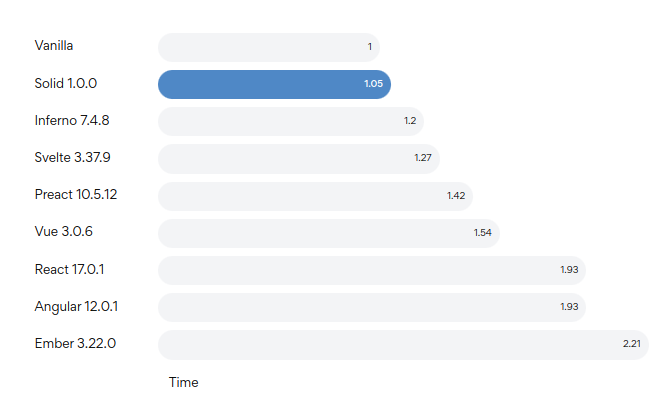
\includegraphics[width=1\textwidth]{solidjs_perf.png}
  \label{solidvsworld}
  \caption{SolidJS vs Other frameworks performance: Taken from~\cite{solid}}
\centering
\end{figure}

There are some disadvantages of SolidJS, most of these come from the very reason that makes it good, the lack of a virtual DOM. Because Solid, needs to update the real DOM programmatically, you need to carefully understand how solid components actually re-render, otherwise the application might not update in some scenarios. \\

Even though Solid is generally harder than React because it does not re-render as often, its very developer friendly APIs and brutal performance, make it the obvious pick for a performance based project such as this.

\subsection{Building and bundling}
As mentioned above, most modern web frameworks (React and Solid included), use JSX. This is great for the developer as it leads to quicker development and more maintainable code, however browsers do not natively support this syntax, and therefore the entire application must go through a stage of transpilation (Taking the JSX into regular JavaScript), and then bundling the application into a few JavaScript files which contain all of the components of the application. Therefore, I must use a tool which both transpiles the code and allows me to build it into a bundled JavaScript file which my end users can then interact with.

\subsubsection{Webpack}
Webpack~\cite{webpack} is the industry standard tool to perform these functions, it is written in JavaScript and takes your code and outputs bundled, transpiled JavaScript files. Webpack has extensive configuration which allows the developer to really specify what settings they want (What version of JavaScript do you need, what poly fills are necessary, etc...). Webpack also provides a development server, allowing me to quickly view my application without having to completely build it. \\

Webpack is great, but there are a few drawbacks. First of the webpack configuration is notoriously difficult to setup, there are many options to choose from and a lot of pre-exiting knowledge is needed is order to create a good webpack configuration. \\

Another drawback is that it is written in JavaScript. JavaScript is great for web application but for intense workloads such as bundling and transpilation, it has weaker performance than compiled languages, making the developer experience here, slower and often less pleasing.

\subsubsection{Vite}
Vite~\cite{vite} is a newer build tool, which provides transpilation, bundling and a development server. Vite uses various other tools to complete these tasks and brings them to the developer in a very easily configured tool. \\

Vite also uses ES Modules, which is a newer browser feature which allows JavaScript files to import and export from other JavaScript files natively, without needing to go through a bundling stage. This means that the Vite Development Server is the fastest amongst tools like it, because it uses ES Modules directly, meaning it only needs to transpile the JavaScript files, but does not need to bundle them. It also allows for Hot-module replacement, which means that when a component changes, you replace that singular component and leave the others unchanged, increasing development speed drastically, because you don't need to wait for a long build time each time you make a change. \\

Vite also integrates very easily with React, Solid, or most other JavaScript frameworks. Making it often a 5 second step to get started with Vite with any of these JavaScript frameworks.

\subsection{Typescript}
JavaScript is the language that browsers use to make websites reactive, paving the foundation for web applications, and most user-facing applications. However, as web applications grew in size and responsibility, it became harder to develop applications which interact with complex data, because JavaScript does not natively support types, as it is a dynamic language, you often don't know the type of something and must perform extra validation in order to make sure data is of the format you expect. \\

This is where Typescript~\cite{typescript} comes in. Typescript is JavaScript with types, it extends Javascript by including interfaces, type declarations and even classes, each with specific fields. This makes working with complex data much easier as the developer is able to know the format of the data, as well as when they have made a mistake with specific objects. \\

Typescript compilers down to regular Javascript, but the compiler is strict and will not compile if it detects type errors, avoiding many of the mistakes that web developers face when building web applications. It also makes the code base much more maintainable, due to other developers knowing exactly the shape of the data they are interacting with. \\

Vite uses ESBuild~\cite{esbuild}, which is a build tool written in Golang, in order to compile the Typescript down to Javascript. This results in extremely fast developing time, even though your code has to go a compilation stage from Typescript down to regular Javascript \\

\pagebreak
\section{Designed Architecture}
One of my projects main goals is to have a scalable architecture, which can automatically scale depending on load from the end users, I needed to create a robust architecture, by splitting the project into smaller systems (micro services) which all work and communicate together.

My project is split into the following (micro) services:
\begin{itemize}
  \item Authentication - User authentication.
  \item Hub - Initial point of contact for users.
  \item Brain - Permanent storage and data management.
\end{itemize}

Each of these services has their own database, as to reduce the dependency on a shared database, therefore increasing the autonomy of each service and increasing scalability as it decouples each system from the others. There is also the downside that, if systems start to share database we begin to lose the source of truth for various events, so if the Hub directly modified the Brain database, the Brain service cannot know how this was changed, and in what context. Below I go into further detail on each of these systems, I have also included a system diagram \ref{architecture}.

\begin{figure}
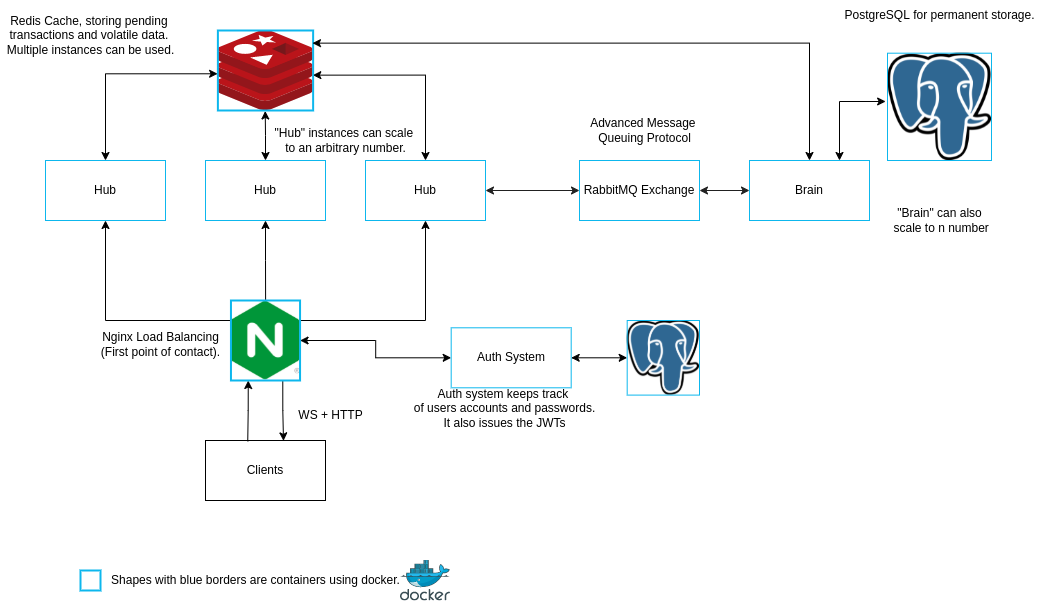
\includegraphics[\textwidth, scale=0.4]{Architecture.png}
  \label{architecture}
  \caption{The backend infrastructure of my system, showing how multiple instances could be used and how different systems communicate with each other}
\centering
\end{figure}

\subsection{Authentication}
This system is the most isolated from the others. As you can see on the diagram is only communicates with the load balancer which comes straight from the user. This is because communication to and from the authentication system contains very secure information such as passwords and access tokens, which if intercepted can allow users to access another users account. Therefore I don't want to handle this information for longer than I need to and definitely through the least number of systems possible - like this we go from the user to Nginx (A load balancer), straight to my authentication system. The specifics are described in this figure \ref{auth_tables} \\

The authentication system has its own database with a few tables that store user information. The database I choose is PostgreSQL, which as outlined in my plan, is one of the fastest, most robust and safest permanent storage databases in the world, often outperforming competition by magnitudes or performance. The tables for this database are as follows: \\

\begin{figure}
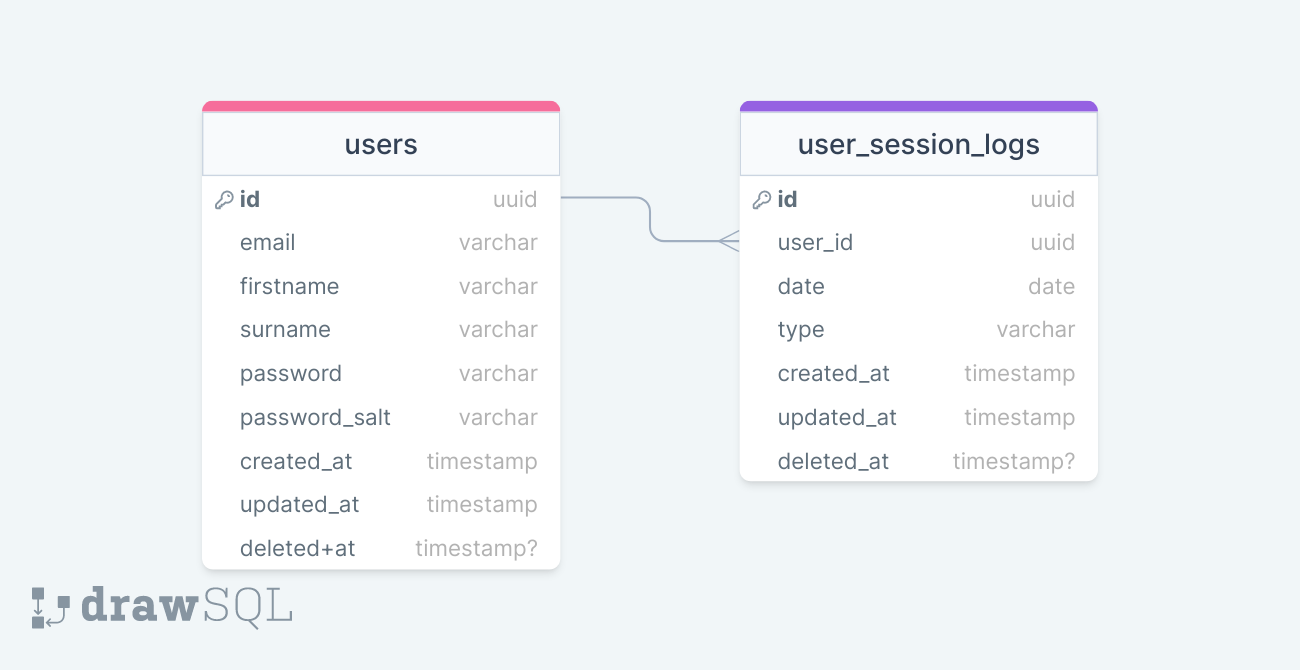
\includegraphics[width=1\textwidth]{auth_diagram.png}
  \label{auth_tables}
  \caption{Authentication system database tables}
\centering
\end{figure}

\subsection{Hub}
The hub is the only service without any permanent storage and this is very intentional. Its job is to act as a router for other services, but also a cache. My aim is to have this service serve from cache around 50 percent of the time. The hub communicates with a Redis database which is a key pair in-memory database, which acts as a very fast caching system, that stores frequently requested data, as to avoid requesting this data from other systems. \\

The Hub can be vertically scaled very easily, together with the Redis database that it users, as Redis supports vertical scaling in a cluster mode. It is likely the system that will be scaled the most, as it will handle all of the users request (except for authentication).

\subsection{Brain}
A terrible name, but the Brain performs CRUD operations on the assets and transactions for the entire system, it acts as an API which the Hub can communicate with to fetch information from. The Brain like all other services has a database of its own, another PostgreSQL database, with the following schema \ref{brain_tables}. The Brain can also scale vertically just like all services but it's difficult to scale the PostgreSQL database vertically because it is difficult to split the data, instead a horizontal scaling approach will be required for the database portion of this service. \\

The brain also communicates with the Redis cluster which the Hub primarily interacts with. This is to update the cache so that the Hub can in future requests return data from this cache database instead of requesting the data from the Brain. The reason I do this step in the Brain service instead of on the Hub on return of the data, is because I want the Hub to only be concerned with handling user requests and either returning the data from cache, or handing it off to another service, as to not "Hold up the line". \\

The main database for the system is in the same service as the Brain. This is a PostgreSQL database which stores the permanent information required through the rest of the application. The schema for this is the following diagram. \\


\begin{figure}
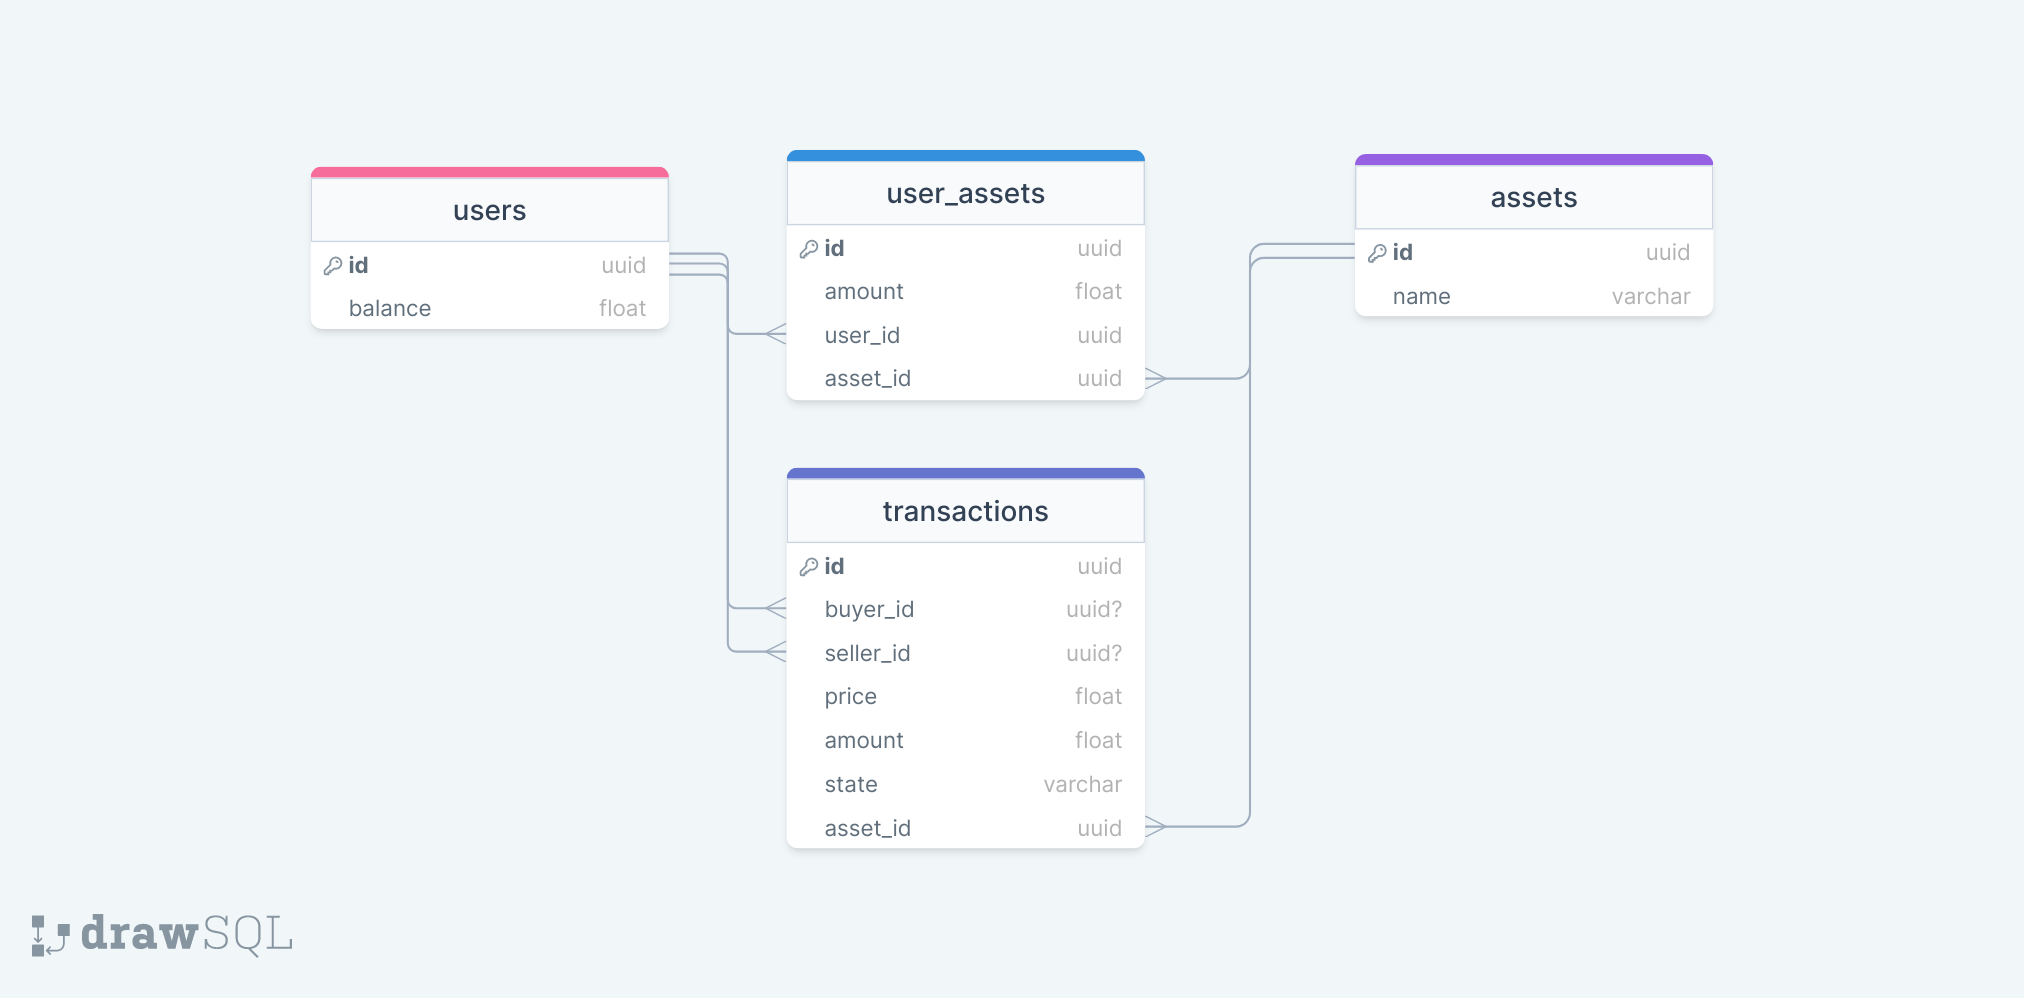
\includegraphics[width=\textwidth]{brain_diagram.png}
  \label{brain_tables}
  \caption{Brain system database tables}
\centering
\end{figure}

All of the tables in the brain database also contain the fields: created\_at, updated\_at and deleted\_at, the same as the authentication system.

\subsection{Communication and Load Balancing}
I have not yet described how these systems communicate with either one another or the user. To start with the user makes request to Nginx which can act as a very high performance web server, load balancer or reverse proxy. These requests are HTTP(s) requests (and also WS), and therefore this is what the Hub receives from the user. \\

However, for the hub to communicate with the Brain service it does not use HTTP requests as these would be somewhat inefficient and not complex enough to handle some of the required distributed behaviour of the systems, therefore I am using RabbitMQ to communicate between the Brain service and the Hub. RabbitMQ acts as a message exchange which supports AMQP (Advanced Messaging Queue Protocol), and with this I can create a sort of RPC (Remote Procedural Call), from the Brain service. All whilst allowing many messages from multiple instances of both services. \\

Micro services architectures generally have the problem of transmitting information across each other, efficiently. To mitigate this problem I have created a library which is shared across my multiple services, that includes the types for commonly used objects. This makes it much easier to share data across system because each one knows the shape of the data, and can easily encode it and decode it without many problems.

\pagebreak
\section{Technologies used}
I have a variety of technologies for my project, these include frontend technologies to create a state of the art web interface, to backend technologies that allow the project to be scaled to as many users as it needs to be scaled to. \\

\subsection{Databases}

\subsubsection{Permanent Storage}
One of the main technical challenges of my project, is choosing the correct database systems. My project requires performance first and foremost and therefore the main consideration when choosing a database is speed. My system also contains highly relational data spread across various areas. Users, assets which user owns which assets and what amount, all this data would be best representation in various table, and therefore SQL Relational Databases seem to be the way forward, the two most popular being: MySQL and PostgreSQL. After researching their features and performance~\cite{postgres_vs_mysql}, I have seen that PostgreSQL reliably beats MySQL in most performance tests, with an even more functionality, making this an obvious choice, for my permanent storage solution. \\

There is another paradigm of databases that have in recent years gotten a lot of transaction, these are document databases. Document databases have much more flexibility than relational databases because they do not (often) contain a set schema, and allows the programmer to easily add/remove parts of data without many constraint. After reading this chapter~\cite{relational_vs_document}, it is clear to me that applications often have a disconnect from the data on the database and the data they actually require in the application, hence why many solutions turn to Document Databases, as these tend to be flexible and de normalisation is common practice. However these databases have poor (or often no), support for joins across tables/collections making one-to-many or many-to-many relationships more difficult. \\

Furthermore, one of the most popular and advances document databases available is MongoDb~\cite{mongodb}, which uses JSON as a method of storage, and has support for data sharding (Splitting into multiple nodes), and (as most document databases do), does not require a schema, giving a lot of flexibility to the developer. However, as shown in this paper~\cite{mongo_vs_postgres}, MongoDb performs worst than PostgreSQL in almost all performance tests, often by some great magnitude. \\

This is one of the easier decisions in the project, I am using PostgreSQL as my permanent storage database(s).

\subsubsection{ORM - Object Relational Mapping}
\label{orm}
In complex project such as this one, it is often not enough to just run raw SQL statements on the database, the reason for this is because of how unmaintainable it is, do you keep them in plain text? What about parsing the data into structures? For these reasons I have decided to use an ORM (Object relational mapping) library, and the most popular one for Golang is Gorm~\cite{gorm}. Gorm allows you to write SQL statements through a builder API, which is fully managed by GORM. \\

GORM just like other ORM, allow the data from the database to be read into type definitions from inside the code itself, in Golang this means structs, this figure \ref{gorm_orm} shows how GORM does this. As you can see we have a normal Golang struct definition but also some annotations, telling us how the struct should behave, in terms of Gorm, it allows us to specify primary or foreign keys easily.

\begin{figure}
  \begin{verbatim}
type User struct {
	Base
	Balance          float64       `json:"Balance"`
	UserAssets       []UserAsset   `json:"UserAssets"`
	BuyTransactions  []Transaction `json:"BuyTransactions" gorm:"foreignKey:BuyerId"`
	SellTransactions []Transaction `json:"SellTransactions" gorm:"foreignKey:SellerId"`
}
  \end{verbatim}
  \caption{GORM type mapping example}
  \label{gorm_orm}
\end{figure}

\subsubsection{Caching}
Caching is a common technique to store commonly used items of data, in a faster, readily available way. For this I am using an in-memory database called Redis~\cite{redis}.

Redis is an unstructured key-value pair in-memory database. Because it is in-memory, it is magnitudes faster than any persistent storage database, therefore I have used it as caching in my system, storing popular assets and data that is used frequently. \\
However, it is important that all the data stored in Redis, can be lost. This means I first have to store it in permanent storage, and only then store it for use in Redis. \\

\subsection{Backend Technologies}
These are the technologies which I used to build the backend system, which consists of the Hub, Brain and Authentication. \\

\subsubsection{Golang}
As a backend programming language I have used Golang , it is a statically typed compiled language, known for its simplicity and ability to write extremely scalable systems, doing my own research I have found that a lot of modern architectures use Golang Real-time Trading Platform \\

Golang is a relatively new programming language that was designed at Google to fit the gap in programming languages for a language that can be adaptive for cloud native use cases, which my system would be. This book~\cite{andrawos2017cloud} describes Golang and its use in cloud computing in more detail but I will state my main reasons for using this programming language.

\begin{itemize}
  \item Concurrency - It is extremely easy to manage concurrent applications in Golang, simply by using a 'Go routine', which means the developer can focus on building the application instead of thinking about concurrent models.
  \item Compiled - Unlike other popular languages in the cloud micro service space such as Node.js~\cite{nodejs} or Python~\cite{python}, which are interpreted and therefore have an overhead in their runtime, Golang compiles down to any desired machine code, making it inherently more performant.
  \item Simplicity - Unlike Java or Scala, Golang does not have classes, which are typically used when a program becomes complex enough that these organizational methods are needed. Golang only includes structs, which are similar to the structs in C. This makes programming declarative and very pleasant to write.
  \item Garbage Collection - Most other competitors also have a garbage collection system, however Golang's garbage collection does not involve a virtual machine (like in: Java, JavaScript, and python). Garbage collection is extremely efficient in Golang.
\end{itemize}

\subsubsection{RabbitMQ}
RabbitMQ~\cite{rabbitmq} is a message broker. It allows various systems to communicate with each other through a reliable and scalable broker, which can be accessed from various system. RabbitMQ is capable of broadcasting messages across systems or simple declaring queues which can be queued and dequeued from the various services accessing it. I am using RabbitMQ to organise the communication between the Hub and the Brain service in my project, mostly due to RabbitMQ supporting multiple clients accessing the queue at a time, meaning that I can have multiple instances of the Hub and Brain both pushing and pulling from the defined queues without much problem.

\subsubsection{JWT}
JSON Web tokens or JWTs for short, are cryptographically safe methods of client side authentication. A JWT is generated in the Authentication system, and signed with a private key, every time the user wishes to authenticate themselves, they serve the JWT to any system, and if the signature on the JWT is correct then the user is authenticated, if not, we know the user either tampered with the signature or it isn't a valid JWT. JWTs can only encode a small amount of data in them, ranging from user information and ids, however this information is accessible to anyone who views the JWT, so it is important that the data is public knowledge. \\

I choose to use JWTs instead of cookie because they are very safe but still quite practice. Like this I do not need to store cookies in the database and check every time against a database that the user is logged in, reducing the amount of lookups various systems would have to perform.

\section{Software Engineering}

\subsection{Methodology}
There are various methodologies used in software engineering, but most of them focus on working with a team of various developers, as well as the client for whom you are making the software. But this is an individual project so I could not simply adopt an Agile strategy or an Extreme Programming strategy, as they aren't applicable to software being developed by one person. However there is a strategy called Rapid Application Development (RAD), which is similar to agile, where it takes an iterative approach to developing software, but excludes daily stand-ups with other teams members, which there obviously aren't any. RAD starts off with a set of requirements which I have outlined in my plan, and it starts a loop of development, taking each feature from design to development. The reason that I chose this methodology is because it allows be to start with very little functionality and iterate over these features until they are complete, or until I run out of time. Because of this I am able to build a POC (Proof of Concept), quickly, and later on iterate over the feature built in order to perfect them.

\subsection{Project Management}
My project is quite complex and has a lot of moving parts which all have different criteria and different objectives. This will be a big challenge, so I will need to employ a good project management strategy if I want to keep on top of everything, and understand the complexity of my project.

For this I will use an app called Todoist~\cite{todoist}, which allows you to have Projects and labels, priorities and deadlines for various tasks. In Todoist (which I have used for a long time to manage almost everything in my life), I have implemented the system from Getting Things Done by David Allen~\cite{gtd}. This is a productivity/organisational system which involves splitting your tasks into lists and project, as well as review and process them in an appropriate manner.

\subsection{Version Control}

\subsubsection{Monorepo}
For this project, we were provided with 1 GitLab repo, however my project consists of various different services and parts that normally would not belong in the same repo. However, there is a common technique in industry of keeping all your code base in the same repository (monorepo), hence making CI (Constant Integration) and development easy, because everything is in one place and not scattered across multiple different project repositories. 

\subsubsection{Bare repo and Worktrees}
Git has a feature called worktrees, this feature is not very well known, however I think it is a very powerful feature and one I have used through this project. Starting with cloning a bare repo, this means that we clone a Git Repository without cloning any of the files in the folder, with the main branch checked out. However, a bare clone just clones the .git file without any of the files, and we can use worktrees to edit various branches, worktrees are a way to have multiple branches in a git repository checked out at the same time, in separate folders. This feature is very powerful because I was often working on 2 things at the same time (Frontend, backend and maybe the report), and naturally these live in different branches, therefore it is extremely useful to have them all checkout out at the same time. 

\subsection{Testing}
Testing is an important part of the software engineering process, and there are various different types of tests which need to be conducted in order for an application to be ready to go out into the wild. It is also important to test the system as a whole with all the spinning parts available.

\subsubsection{Unit Testing}
Unit testing is the most basic type of testing, it consists of isolating specific functions/files and testing their functionality. I find that in a distributed system these tests are the most useless out of all tests, and therefore I will give less energy to them. This is because the most important part in my system is to test the overall behaviour of all the services and not the individual behaviour. This is not to say unit tests are not important, they are, but in my case they will be the least important. \\

I am using Golang's built in testing library, which consists of writing test files with the \_test.go postfix, and using the Golang CLI to run the tests. \\

For the frontend I am using Jest~\cite{jest}, which gives you testing utilities for testing Javascript projects, and I will also use Solid Testing Library~\cite{solid_testing}, which provides utilities for testing SolidJS components specifically.

\subsubsection{Integration Testing}
Integration testing includes the testing of an application or multiple applications running together, but falls short of the entire system. In my project, the Hub and Brain system would need integration tests because these systems work very close together. \\

In my project I created a subproject dedicated to integration testing with the backend system, this includes API testing down to the route level, creating mock data for the database and expecting a certain amount of data returned at each endpoint. Below is a snipped from my integration testing, for a route which should return assets in the system.

\begin{verbatim}
  it("Should give error on non-registered account", (done: jest.DoneCallback) => {
    request(AuthUrl).post(l).send({
      email: "notregister@email.com",
      password: "password",
    }).expect(400).end((err, res) => {
      expect(err).toBeNull();
      expect(res.body).toMatchInlineSnapshot(`
        {
          "error": "this account doesn't exist",
        }
      `);
      done();
    });
  });
\end{verbatim}

Just like any good test, these tests are automatic, and describe themselves. I am making a request to the Authentication Url, sending some data and expecting certain data to come back to me. \\

\subsubsection{End-to-End Testing}
End-to-end testing is the closest to the real world. These tests are mostly (but not always), done on the frontend application, because this is where the user would interact with the system from. The purpose behind these tests is the test the overall functionality of the system, without worrying about any of the details. \\

Testing frameworks for this type of testing often consist of opening an actual browser window and clicking various parts of the UI to see if they work as intended, to help me do this I will use Cypress~\cite{cypress}, this framework allows me as the developer to very quickly write end-to-end tests and provides the test runner and UI to show me how the tests are running, as well as where the tests are failing. 

\section{End system development}
I have talked extensively about decisions I made during the design stage of the project, the research that went into these decisions and why I have layed out the architecture the way I did. I have not yet talked about what the system currently does, what features and goals I have achieved, and how I will continue to work on the project to bring it to completion. \\

Each system has its own Dockerfile which is used in the docker compose file that starts all the systems and databases.

\subsection{Authentication System}
The easier part of my project was building an authentication system, which allowing for registering and login, as well as refreshing the users authentication. To authenticate the user, the user must provide their email and password, after which they receive a JWT~\cite{jwt}, which proves to the other systems who the user is, and allows other systems to also prove that the user is who they say they are, because JWTs are cryptographically safe. \\

The user is issued 2 JWTs. A "refresh" token and an "access" token. The refresh token can only be used in the /refresh API Route, all it does it allows the user to get another "access" token, because it doesn't actually allow the user to access any of the other systems, it has a long lifespan (time for which it is valid), of 2 weeks. This also means the user can be logged in for up to 2 weeks at a time without having to login again. The access token grants the user access to the entire system, and because of this it has a very short lifespan of 5 minutes, again these can only be obtained when first registering or logging in, and subsequently using the /refresh endpoint, which issues a new access token. \\

The authentication system is implemented in Golang, just like the rest of my backend services.

There are 3 endpoints in the authentication system:
\begin{itemize}
  \item /register - Allows users to register a new account.
  \item /login - Allows users to login with their pre-existing accounts.
  \item /refresh - Refreshes the users JWT, using a refresh token.
\end{itemize}

This system is fully complete, and testing using integration tests which I will discuss later. There shouldn't be any need to make changes to this system in the future.

\subsubsection{Dockerfile}
\begin{verbatim}
FROM golang:1.19.3-alpine3.16
WORKDIR /auth
ADD ./auth .
COPY ./shared-types ../shared-types
COPY ./utils ../utils
RUN go build -o auth
EXPOSE 4546
CMD [ "/auth/auth" ]
\end{verbatim}

\subsection{Hub System}
The hub system takes in all of the user communication (except for authentication requests). As it stands it has an API, which allows the users to access assets, and create transaction requests. This means that most of the features for the system are actually implemented. However, as it stands the system currently lacks any sort of caching and always makes RPC calls to the Brain service to retrieve information, this is not efficient as is something I will work on as soon as the presentation is complete. It is also written in Golang and has the following endpoints:

\begin{itemize}
  \item /health - Checks if the system is responsive.
  \item /assets - Lists all the assets.
  \item /trade - Lists all the currently open trades.
  \item /trade/create - Creates an open trade (buy/sell).
  \item /trade/complete - Allows the user to complete an open trade from another user and buy/sell whatever the other user was buying/selling.
  \item /users/assets - Returns the assets owned by the user.
  \item /ws - Allows the user to upgrade their connection to a WS connection.
\end{itemize}

As it stands this service also doesn't provide updates using WebSockets, which means it needs to be constantly asked about pending trades and listing assets. This is not great because it creates extra load on the service, and also a slower experience for the user. The infrastructure is there to allow WebSocket connections and updates, however I have decided to hold off on fully implementing this in order to get the core features done, which I have.

\subsubsection{Dockerfile}
The Dockerfiles are quite similar to one another, the only thing being different is the port. This is mostly because they are all Golang application that all include the shared libraries I created to facilitate development.
\begin{verbatim}
FROM golang:1.19.3-alpine3.16
WORKDIR /hub
ADD ./hub .
COPY ./shared-types ../shared-types
COPY ./utils ../utils
RUN go build -o hub
EXPOSE 4545
CMD [ "/hub/hub" ]
\end{verbatim}

\subsection{Brain System}
The brain system handles the saving and retrieval of permanently stored data relating to users transactions and assets. It receives requests from the Hub system and responds to them with the corresponding database data. It uses RPC to do this together with RabbitMQ. I will talk about this below. \\

To allow for better communication between the two systems I have a shared types library which is included in both system, so that they can easily exchange data and know the shape of said data. Currently this system can perform Create and Read operations on users, users assets, assets and transactions and return them to the Hub, so they can be on their way to the user.

\subsubsection{Dockerfile}
\begin{verbatim}
FROM golang:1.19.3-alpine3.16
WORKDIR /brain
ADD ./brain .
COPY ./shared-types ../shared-types
COPY ./utils ../utils
RUN go build -o brain
CMD [ "/brain/brain" ]
\end{verbatim}

\subsection{RPC Communication}
RPC (Remote Procedural Call), is a mechanism to make calls to functions that do aren't on the program calling them, this is very useful in my micro services architecture because I want to retrieve data from other services in an easy and convenient way. To do this, I have made use of Golang's Go Routines and RabbitMQ as the message broker where the messages are sent to and pulled down from. \\

When a services requests an RPC, they publish a request to RabbitMQ RPC Queue, which has declared when the services started up. Whilst this is happening any service that should receive RPCs, waits for an event to be pushed onto the RPC Queue, this waiting occurs in a Go routine, which in this case is just another thread, this is done so checking for new messages and regular program operations can both happen concurrently. When a new event was published to the RPC queue the Go routine picks up on it and perform the required function asked by the request, after it's done it send an event to the Callback Queue with the same Id as the call received, this means in the other service that made the RPC call, we can do the same type of waiting, and check if an event with the same Id was received in the Callback Queue. A diagram that better illustrates this is below:

\begin{figure}
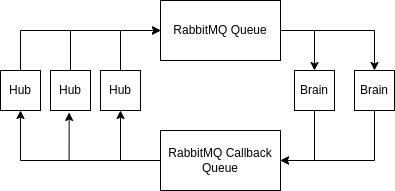
\includegraphics[width=\textwidth]{RPC.png}
\caption{Remote Procedural Call between Hub and Brain Services}
\centering
\end{figure}
\pagebreak

\subsection{Shared Types and Utilities}
As I mentioned before I have created a library which contains the types that are meant to be shared across the entire system, these create a consistent standard of communication across services, which can often be difficult to assert. This way, we have 1 source of truth for what the data should look like, all included in a package that all services have access to. \\

I have also created a utility package which contains functions that are used throughout the application, these include JWT verification, and middlewares used in multiple services. 

\pagebreak

\subsection{Docker Compose}
The docker compose file contains all the information for the entire system, it also includes the databases for each of the systems and the RabbitMQ service that is started alongside them. It also specifies information such as network mode, restarting behaviors, contexts etc...

\begin{verbatim}
version: "3"

services:
  rabbitmq:
    build: ./rabbitmq
    ports:
      - 15672:15672 #Management console
      - 5672:5672 #Actual exchange
    network_mode: host
    restart: on-failure

  # Hub service is the entry point for all thing (except authentication)
  hub:
    build: 
      context: .
      dockerfile: ./Hub.Dockerfile
    ports:
      - 4545:4545
    depends_on:
      - rabbitmq
    restart: on-failure
    network_mode: host

  # Brain service consumes RabbitMQ request and deals with permanent storage
  brain:
    build: 
      context: .
      dockerfile: ./Brain.Dockerfile
    ports:
      - 5672:5672
    depends_on: 
      - brain_postgres
      - rabbitmq
    restart: on-failure
    network_mode: host

  brain_postgres:
    build: ./brain_postgres
    volumes:
      - ./brain_postgres/scripts/init.sql:/docker-entrypoint-initdb.d/init.sql
      - ./brain_postgres/db:/var/lib/postgresql/data
    environment:
      - POSTGRES_NAME=postgres
      - POSTGRES_USER=postgres
      - POSTGRES_PASSWORD=postgres
    healthcheck:
      test: ["CMD-SHELL", "pg_isready -U $$POSTGRES_USER"]
    ports:
      - 5443:5432

  auth:
    build: 
      context: .
      dockerfile: ./Auth.Dockerfile
    ports:
      - 4546:4546
    depends_on: 
      - brain_postgres
      - auth_postgres
    restart: on-failure
    network_mode: host

  auth_postgres:
    build: ./auth_postgres
    volumes:
      - ./auth_postgres/scripts/init.sql:/docker-entrypoint-initdb.d/init.sql
      - ./auth_postgres/db:/var/lib/postgresql/data
    environment:
      - POSTGRES_NAME=postgres
      - POSTGRES_USER=postgres
      - POSTGRES_PASSWORD=postgres
    healthcheck:
      test: ["CMD-SHELL", "pg_isready -U $$POSTGRES_USER"]
    ports:
      - 5442:5432
\end{verbatim}

As you can see the docker compose file is quite extensively because it has to contain the various services used for my project, it runs the RabbitMQ service, various databases and all the services which I have coded. It also configures ports and environment variables as well as docker volumes.

\pagebreak

\section{Methodology}
In this section I will discuss my uses of software engineering tools and techniques that I used in order to deliver on the project.

\subsection{Using Git and GitLab}
By far the most important tool that I used throughout my project was Git~\cite{git}. Git is a distributed version control system that allows code to be stored in a way that it can be searched, checked out, branched and many other features. \\

In my project I took liberal use of branching from a main branch, where all features were developed from. There are times when I pushed a commit straight into the main branch but mostly this was small configuration changes that did not require much in terms of features, which for a solo project is fine. Below I have entered a visualization of my git branching history, visualized using the following command: git log --graph --decorate --oneline.

\begin{verbatim}
* f1645ef (HEAD -> report-perf-evaluation, origin/report-perf-evaluation) 
  REPORT: Adding heading that I plan on writing
* fd1b155 REPORT: Finished the virtual machine white box testing evaluation
* c954611 REPORT: Adding performance evaluation (login route)
*   007612c (origin/main, origin/HEAD, main) 
    Merge branch 'performance-testing' into 'main'
|\
| * b9e2feb FEAT: Adding get trades chart
| * f06326c FEAT: Adding get trades testing
| * f88d054 FEAT: Testing cache invalidation
| *   8468f4f Merge branch 'main' into performance-testing
| |\
| * | 0124b80 FEAT: Complete trade testing
| * | a723bcc FEAT: Login route and create trade testing complete
* | | 9827468 FIX: There wasn't really an issue it seems
| |/
|/|
* |   4b0dd8e Merge branch 'fix-buy-bug' into 'main'
|\ \
| * | ff7145e CHORE: Adding comment to unclear code
| * | 8c7282e FIX: A user can no longer trade with themselves
| * | dcc8606 FIX: When the user bought without already owning some,
      db wouldn't save new asset
* | |   bbb20e1 Merge branch 'frontend-requests-refactor' into 'main'
|\ \ \
| |/ /
|/| |
| * | 59f6e96 REFACTOR: Util function to set tokens
| * | dbbe94e FEAT: Using suspense to wait for user authentication
| * | 6a3bf7e REFACTOR: Login and register pages logic
| * | 08dc5f6 WIP(auth): Refactoring the frontend authentication code
| * | e9c6cae CHORE: Removing unnecessary console logs
| * | 1b6a918 REFACTOR(requests): Using axios create client
|/ /
\end{verbatim}

As you can see, the development occurs on separate branches from main, and often take place in parallel because of the amount of different features throughout my project. As you can see, there are also places where the main branch is merged into my feature branch, this is because I would often merge features into the main code base and then it is good practice to always work with the most up to date version of the trunk, or in this case the main branch. \\

Through the beginning of my project I simply used Git on its own to manage my project, however towards the end stages of developing the project I ran into the limitation that I was working on multiple features at the same time, and these can be managed just fine by Git, but it is difficult as an engineer to context switch between these features whilst maintaining a good level of code quality. To help solve this problem I looked at GitLab's~\cite{gitlab_cite} own merge request environments. Instead of merging into main using regular terminal Git commands, I started a merge/pull request on GitLab, and would use that environment as a hub for the code, where I would often leave comments to myself and do some code review of my own code. An example of this is shown in this figure \ref{gitlab}. \\

\begin{figure}[h!]
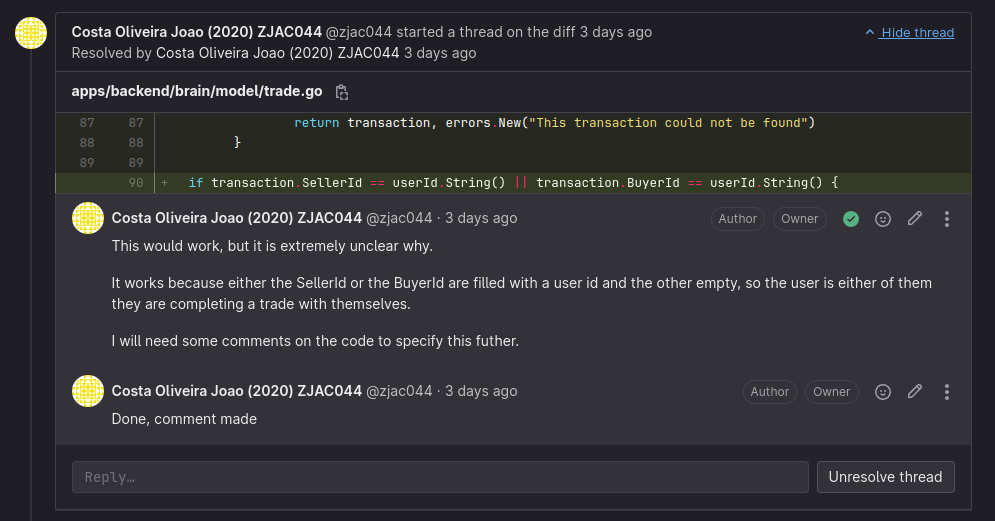
\includegraphics[width=\textwidth]{../Diagrams/GitLab.png}
  \caption{GitLab Code Review Example}
\label{gitlab}
\end{figure}

This might seem strange at first, after all these features were designed with a team of engineers in mind and not just a single person, however I found that having a space to make myself accountable to myself was extremely useful, specially when doing refactoring work towards the end of the project, as often it was not technical decisions that I needed to review, but simply code quality, which is something the figure \ref{gitlab} demonstrates. \\

Another important Git convention which I followed is the commit messages. We know that these must be descriptive to what the commit is doing, however I went a step further in starting all my commits (Bar a handful), with keywords such as: FIX, REFACTOR, FEAT, CHORE, which indicate very clearly to myself what I was working on on certain commits. This convention proved to be so useful to myself that I stopped using the log book which I had stuck to throughout term one because I found myself simply rewriting the commit messages that I had done for the day. 

\pagebreak
\subsubsection{GitLab Runners}
Early on in my project, after setting up docker, I ran into the issue of constantly having to build docker images and upload them to Docker Hub~\cite{docker_hub}. This was not a lot of time, but it was mostly that I would often forget to do this, because it isn't work that a programmer should do it, the task should be automated. So I decided to spend some time and automate it. \\

The universities GitLab instance does not provide CI runners, therefore I had to setup my own Git Lab CI Runner~\cite{gitlab_runner} on my own Virtual Machine (The same virtual machine I used for testing). The process wasn't easy but involved running the CI runner as a docker image which then mostly manages itself. The more complicated part came with the connecting this runner to the universities GitLab instance, and then writing a GitLab CI file to actually compile the images, this file is below.

\begin{verbatim}
stages:
  - build

docker_build:
  image: docker:latest
  services:
    - docker:dind
  stage: build
  rules:
    - if: $CI_COMMIT_BRANCH == "main"
  script:
    - cd apps/backend
    - docker login -u johncosta27 -p $DOCKER_TOKEN
    - docker build -f Auth.Dockerfile -t johncosta27/fyp-auth .
    - docker push johncosta27/fyp-auth
    - docker build -f Brain.Dockerfile -t johncosta27/fyp-brain .
    - docker push johncosta27/fyp-brain
    - docker build -f Hub.Dockerfile -t johncosta27/fyp-hub .
    - docker push johncosta27/fyp-hub
\end{verbatim}

The CI file itself only took a while to write because I wasn't familiar with the configuration and the only way to test it was to push into the main branch and see if it worked (this was one of the few instances where I pushed straight into the main branch). You can see environment variables scattered throughout the file like: DOCKER\_TOKEN. These were sensitive secrets which wouldn't be appropriate to place inside a text file, instead GitLab provides its own secret management system, where I store these tokens, maintaining them away from my Git history. \\

This file worked well, and the runner was very stable and never seemed to crash on the VM, therefore I was able to have an automatic docker image builder which pushed to my docker registry. \\

I also attempted to use the same CI pipeline to run the integration tests. Unfortunately I was not able to do this, because of a lack of expertise in CI environments. The problem was that the runner itself is a docker image, and I was asking it to run a bunch of docker images (my project), and run the integration tests on it. The pipeline went as far as spinning up the images but I ended up with being unable to access the databases, which is obviously a big issue. This was taking up a lot of hours to try and solve and so I decided to abandon this prospect. 

\pagebreak
\subsection{Testing}
Testing in my project was mostly carried out through the testing of API requests instead of unit testing in each function. This decision was made because often services rely on other services in order to run, for example the Hub needs the Brain to read data. If I was to unit test the Hub I would need to create a 'dummy' Brain which I would then need to keep updated with the real brain. This is not ideal because; firstly it is not a realistic test; secondly I would need to constantly change this dummy API every time the real brain is changed, making this unrealistic. \\

\subsubsection{Integration Testing}
Integration tests are the primary tests in my project, these involve running all the backend together, including all the databases, and testing the system by sending HTTP Requests and checking the responses are adequate, this tests access rights, the shape of data, and various other things. \\ 
My integration tests also have a mechanism to clear the databases clean and add testing data so that the tests can stay deterministic. \\

The tests are written using Node.js~\cite{nodejs}, this is purely because it is much faster to write and use from a developers perspective, at the cost of performance. However during tests that are not touched by the user, performance is not a concern. The testing libraries I use are:

\begin{itemize}
  \item Jest~\cite{jest} - Testing framework
  \item Supertest~\cite{supertest} - Builder pattern request builder
  \item Prisma~\cite{prisma} - Type safe ORM, to create dummy data and clear the databases.
\end{itemize}

I have added an example of the tests in the report before, but in this figure \ref{integration} you can see what the results of the tests look like.

\begin{figure}[h]
  \begin{verbatim}
PASS  src/auth/refresh.test.ts
PASS  src/auth/register.test.ts
PASS  src/auth/login.test.ts
PASS  src/hub/assets.test.ts
PASS  src/hub/asset-trades.test.ts
PASS  src/hub/users.test.ts
PASS  src/hub/trade.test.ts

Test Suites: 7 passed, 7 total
Tests:       22 passed, 22 total
Snapshots:   12 passed, 12 total
Time:        3.867 s, estimated 5 s
Ran all test suites matching /test/i.
  \end{verbatim}
  \caption{Integration Tests Results}
  \label{integration}
\end{figure}

Each Node.js project also has a package.json file where you can define scripts to make the running of the project easier, I utilized this to create scripts that make it 1 command to run tests.

\begin{itemize}
  \item npm run test:clean - Cleans the database, creates new test data and runs the tests.
  \item npm run test:run - Just runs the test with the same test data.
  \item npm run prisma:gen - Generates the types from the database to allow prisma to access db.
\end{itemize}

\subsubsection{End to end frontend testing}
To test the frontend application I have used an open-source framework called Cypress~\cite{cypress}. It provides a framework for testing an application from the perspective of the user without having to know about the underlying code, you write tests in a way that describes a user navigating through the website. This is the most real type of testing you can do because of it having 0 knowledge of the working system, it simply clicks buttons just like a regular user would. \\

Here is an example of what a cypress testing file would look like:

\begin{verbatim}
  it('Allows user to see email but not password', () => {
    cy.fixture('users').then(users => {
      cy.get('input').eq(0).type(users[0].email);
      cy.get('input[type="password"]').type(users[0].password);

      cy.get('input').eq(0).should('have.value', users[0].email);
      cy.get('input[type=password]').should('have.value', users[0].password);
    });
  });
\end{verbatim}

The code above is extremely descriptive and uses DOM selectors (Statements that fetch data directly from the HTML of the website), and perform certain assertions on them. Cypress also provides fixtures, which are externally written JSON files that allow you to easily drop in testing data, in this case I am using this feature for getting testing users emails and passwords.

\subsection{Project management}
I started off using Todoist~\cite{todoist} for my project management, however I found that it become quite restricted specially when I had to jump between features, bug fixes and report writing, and I tend to prefer a lot of organisation over the lack of it, therefore I found a project management application which has basic cards, issues, backlogs and most other features that scrum teams use for software development. The tool I choose is Linear~\cite{linear}. In this figure you can see what the current state of the project is as I write this report (most development done, mostly bug fixes and report writing). \ref{linear_example}

\begin{figure}[h]
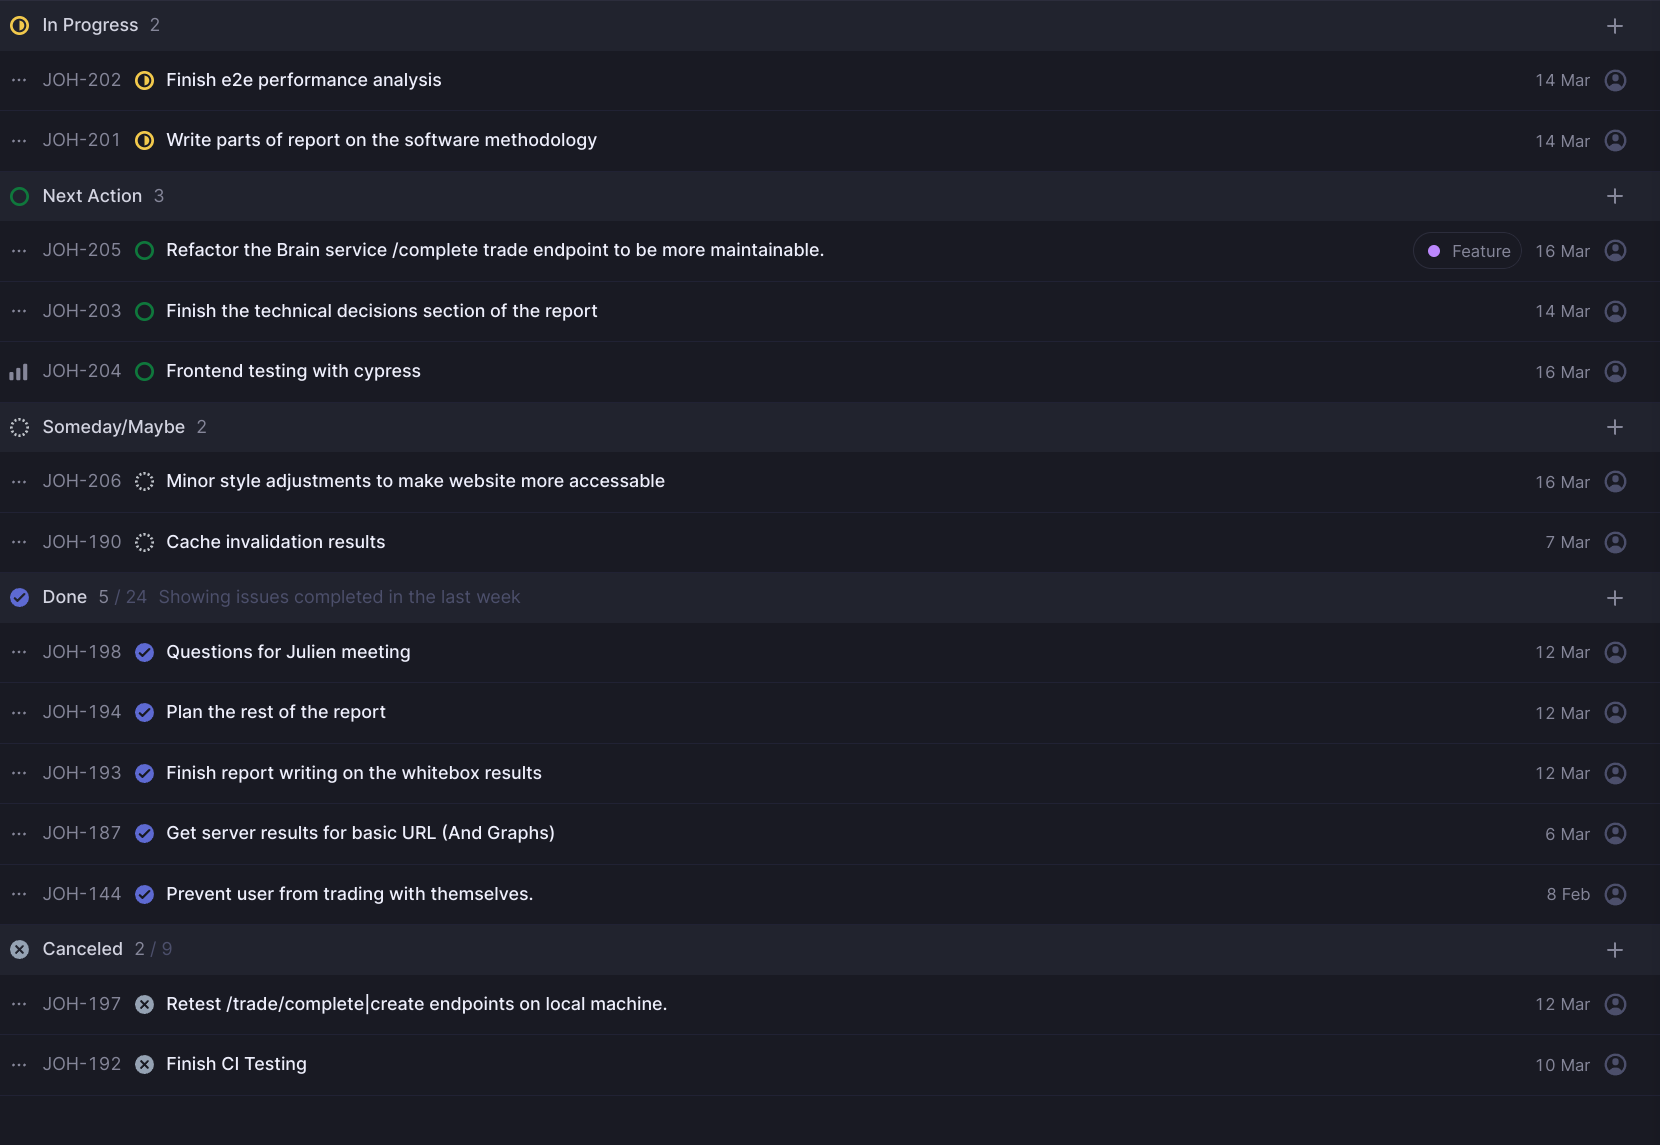
\includegraphics[width=\textwidth]{../Diagrams/linear.png}
  \caption{Linear Project Management Tool}
\label{linear_example}
\end{figure}

As you can see I have 5 sections, which follow the advice given by David Allen in Getting Things Done book~\cite{gtd}

\begin{itemize}
  \item In Progress
  \item Next Action
  \item Someday/Maybe
  \item Done
  \item Cancelled
\end{itemize}

\pagebreak
\section{Technical Development}
\subsection{Backend technical decisions}
The backend of my system is where most of the complexity lies, I discussed earlier on why I have decided to split it into 3 components (Hub, Brain and Authentication), but I will now discuss some more technical details.

\subsubsection{Why RabbitMQ?}
\label{rabbitmq_comms}
For my Hub service to communicate with the Brain service they use an AMQP Queue~\cite{amqp}, which RabbitMQ provides. The reason for this is because of the reliability and versatility of RabbitMQ. It is known in the industry to be extremely reliable and predictable which is important for the stability to my system. \\

I could have instead just used HTTP requests to access the Brain service, but I choose against this because I wanted to control exactly who is communicating with the Brain, instead of having an open API that anyone can access. Furthermore HTTP requests are harder to control and predict when running in multi-node environment (If I have 2 instances of the brain, which one is getting the requests?), this problem can be avoided by using some load balancer, but I decided to avoid it all together. \\

Furthermore, RabbitMQ has more advanced features such as fanout exchanges, which allow you to publish messages onto various queues at the same time without ever having to manage this complexity, I am not using this in my system currently, but it could be a feature I took advantage of in the future.

\subsubsection{Queue per service system}
\label{one_queue}
Every node on my system has an attached RabbitMQ queue. So the Hub service has a queue which other services can push items onto and the Hub will process these accordingly, it is important to note that this queue is unique to the instance of the service, so it is easy to know which instance is actually handling which parts of the requests. \\

This decision comes at the cost of having to manage multiple queues in the system and manage IDs for these given queues. I talk more about how I managed this in the "shared types and utilities" section of the report.

\pagebreak
\subsubsection{Caching}
The Hub service doesn't always have to go to the brain service in order to reply to the client, the reason for this is that I have implemented a caching system using a Redis database that allows me to reduce the response time for request, and generally reduce the load on the system for commonly fetches, but uncommonly changed data. The results for this mechanics are below in the evaluation section. \\

The hard part of caching was cache invalidation. This is the way of taking cache that I believe to be stale and no longer up to date, and removing it from cache so that the Hub service has to go and fetch the up to date information from RAM. \\

The hard problem to solve here has nothing to do with the actual caching itself, but how to decouple the request handling logic, from the caching logic. To achieve this I used a middleware, which is a function that runs when the user sends an HTTP request, but importantly runs BEFORE the request is handled (I use a similar middleware to validate that the user is authenticated). The code for the request is in the following figure \ref{cachereq}.

\begin{figure}
  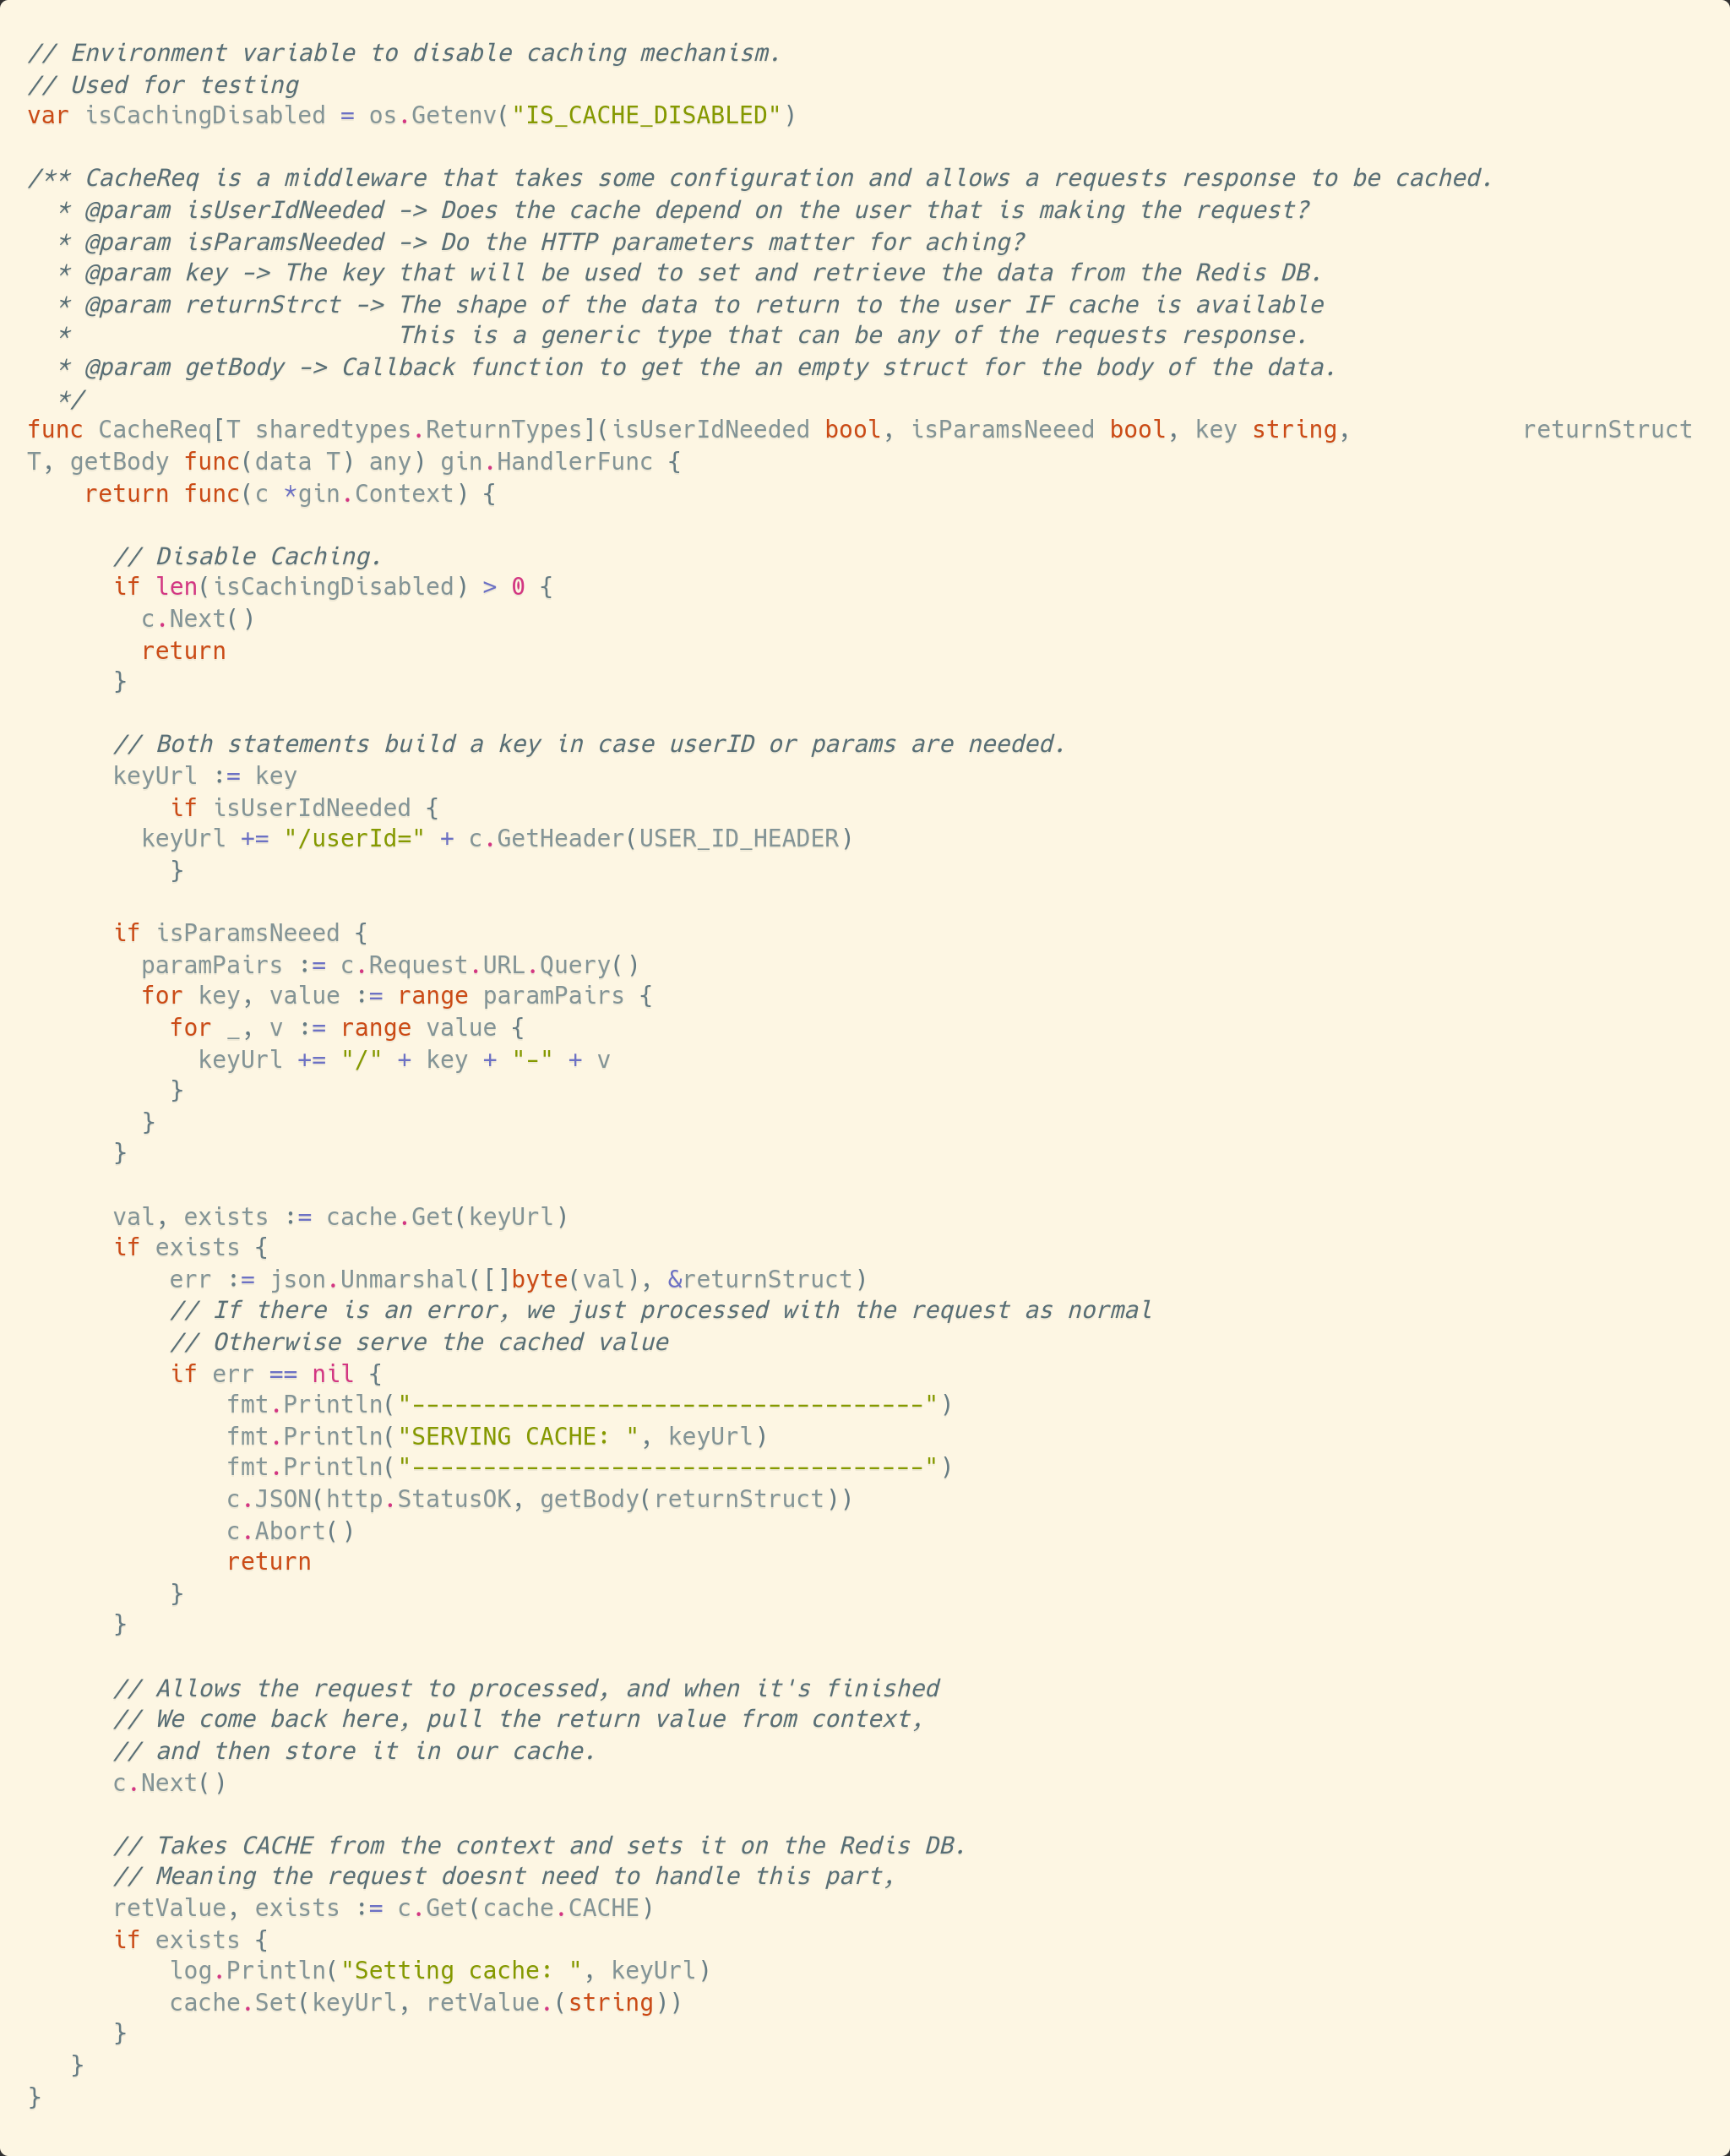
\includegraphics[width=\textwidth]{../Diagrams/cachereq.png}
  \caption{Cache Request Middleware}
  \label{cachereq}
\end{figure}

\pagebreak
\subsubsection{Shared types and utilities}
Because my entire backend systems were written in Golang, and they all involve similar problem, it is only natural that I was going to run into code repetition whilst working on this project. I began tackling this by not tackling it at all within the first few weeks of development, I would often copy various parts of the code into different folders so that I could use it in all the services. This worked because it allowed me to move fast and actually get the work of getting the project started done. However, it came a time where this was a liability. \\

As you are now aware, the Hub service and the Brain service communicate constantly. However, how can I ensure that the format of the data is preserved on either end? Because if I try to parse some data into a certain memory allocation and I get it wrong, the program is going to have a run time error. This is a big problem even in the industry, with many tools to help prevent these. Some of the tools are. \\

CITE HERE
\begin{itemize}
  \item GraphQL~\cite{graphql} - A schema for transmitting and request data across different services.
  \item WebRPC~\cite{webrpc} - Code-generation driven approach to writing schemas for web services.
  \item gRPC~\cite{grpc} - Multi-language RPC framework.
\end{itemize}

Some of the listed solutions are more opinionated than others, but they all had the drawback of having a significant learning curve, and if I was to use any of them I would be simply over-engineering my project. As the project stands now, there is a much simpler solution to the problem of achieving end-to-end type safety, so long as the project remains small. If the project was to be used by more than 2 or 3 engineers, and be seriously developed, I would definitely invest the time and effort into looking into a more robust solution. \\

For now I am simply using a shared types library, which is copied into each of the service's docker images when they are build. This ensures that I have consistent type definitions on every service that requires them, and as long as I stay consistent on type casting into these structs, there cannot be any run-time errors. The figure \ref{sharedtype} shows an example of such type definition. This figure shows the type Transaction, which the Hub requests from the Brain using simple RPC. Because the services communicate using JSON that is turned into bytes, there must be a way of converting the JSON back into a struct, to be used by either side of the events. This solution ensures the consistent typing of data on both ends. \\

You can also the json type annotation, to know how to Marshall and Unmarshall the JSON data and what keys to use.

\begin{figure}
  \begin{verbatim}
type Base struct {
	ID        uuid.UUID  `gorm:"type:uuid;primary_key;" json:"Id"`
	CreatedAt time.Time  `json:"CreatedAt"`
	UpdatedAt time.Time  `json:"UpdatedAt"`
	DeletedAt *time.Time `sql:"index" json:"DeletedAt"`
}

type Transaction struct {
	Base
	AssetId  string  `json:"AssetId"`
	BuyerId  string  `json:"BuyerId"`
	SellerId string  `json:"SellerId"`
	State    string  `json:"State"`
	Price    float64 `json:"Price"`
	Amount   float64 `json:"Amount"`
}
  \end{verbatim}
  \caption{Example of a shared type}
  \label{sharedtype}
\end{figure}

Another part of my project that is shared is a few utility functions, and even the RabbitMQ client which I designed to work specifically for my system. I won't add code snippets here because it is quite extensive, but in my projects 'apps/backend/utils', you will find various pieces of code that are shared throughout my 3 services, the most important one being the RabbitMQ client, which enables the services to send and receive messages through my RabbitMQ system without needing to implement this logic every time.

\subsection{ACID Compliant Transactions}
I have mentioned in an earlier section \ref{orm} the use of ORM, and specifically GORM~\cite{gorm} in my project, and how GORM (An ORM library for Golang, which I used when interacting with databases), uses transactions by default on every create, update and delete statement it performs. However there is one part of my project where this is not so easy because I need two databases to be in sync at the same time. This happens when there is a new user registered into the system. \\

When a user registers themselves onto my system they do so on the Authentication system, then the Brain database must also create a new user with the same ID, this part is crucial for performance because if the IDs were not in sync the JWT what authenticates the user could not be used in the brain, and at best we would have to request the Auth system to validate the JWT and then processed with the request, which adds a lot of internal traffic that can simply be avoided. \\

To avoid this, when I create a user on the Authentication database, I do the same, with the same ID on the Brain database, however a problem arrises - How do I make sure that if one of the databases fails to create a user, we can roll back both databases? The answer comes with the use of manual transactions. We first create the user on the Auth database, use RabbitMQ to tell the Brain service to also create a user, and if an error occurs at any point we roll back the database. Here is a code snippet from the Authentication service where this is done \ref{auth_register_safe}. \\

Ideally, every database is independent from each other, and technically they still are as the authentication service isn't directly communicating with the Brains database (Which is a core principle or micro service architectures), however the complexity of having different user records in different databases for the same user would create too much further complexity than this would, and therefore that is why I choose to do it. But it is the only place in the project where an inter database dependence happens.

\begin{figure}
  \begin{verbatim}
// To create a user we must sync the IDs across databases,
// to facilitate lookups, throughout the system without the need
// of constant communication across system.
// GORM does this by default, but here we need to do this manually
// because of the 2 different databases.

transaction := database.Db.Begin()
res := transaction.Create(&user)

// Early return if the auth database has had an error.
if res.Error != nil {
  log.Println(res.Error)
  c.JSON(http.StatusBadRequest, gin.H{
    "Error": "Duplicate email found",
  })
  transaction.Rollback()
  return
}

// Request the brain to create a new user.
brainResponse := rabbitmq.AuthEventClient.Send(brainReq)

// Get the response.
var isUserCreated bool
err := json.Unmarshal(brainResponse, &isUserCreated)

// Error checking
if err != nil || !isUserCreated {
  log.Println(err)
  c.JSON(http.StatusInternalServerError, gin.H{
    "Error": "There has been a server error creating user",
  })

  // The user was created on the auth database.
  // But not on the brain, therefore we need to rollback
  if res.Error == nil {
    transaction.Rollback()
  }

  return
}

// After all validation, it is safe to commit to database.
transaction.Commit()
  \end{verbatim}
  \caption{Authentication and Brain syncing with newly registered user.}
  \label{auth_register_safe}
\end{figure}

\pagebreak

\subsection{Inter Service Communication}
I mentioned earlier that I have used RabbitMQ for my services to communicate with each other \ref{rabbitmq_comms}. However to communicate with an AMQP queue, takes a fair bit of boilerplate code, and because of this I have created a small shared library that facilitates the attachment of services onto the RabbitMQ messaging service. The code is quite long but can be found at \lstinline{apps/backend/utils/rabbitmq.go}. \\

What it does is allow each service to have an ID, which will be the name of their queue (I have talked about the design decision to have 1 queue per system here \ref{one_queue}). It then connects to RabbitMQ and does all the error and validation checks for you, instead of the developer having to write it out each time. To create a new event client (which is what I called this system), one must also supply two callback functions, one for listening to RPC requests, and another for listening to simple info request, which do not need to supply a response. Interestingly, you can just create empty functions if you do not which the service to do anything when it is requested upon. \\

The event client also supplies basic functions to help with sending RPC communication between services, furthermore it also helps with type safety, because it returns the correct Golang struct each time, meaning that you will get a compile error if you try and send anything except this struct through the system.

\pagebreak

\subsection{Authentication}
Authentication in my system is done using JWTs~\cite{jwt}, which allows users to authenticate themselves with a cryptographically safe token. This token is sent between the client and either the Hub or the Authentication system, it is not required between the Hub and the Brain as this communication is controlled only through the Hub, and the Brain cannot be accessed from the outside world. To validate this token I have create another middleware, that simply checks that the JWT is correct. The figure \ref{authmiddleware} shows an example

\begin{figure}
  \begin{verbatim}
const USER_ID_HEADER = "userId"

/** Middleware to check the authentication of the user.
  * If the user is not authenticated, their request will be returned,
  * with an unauthorized message, and will not processed.
  *
  * If the JWT is safe, then the request will processed as normal.
  */
func Auth() gin.HandlerFunc {
  return func (c *gin.Context) {

    // Fetches the access token from the header of the request
    accessToken := c.GetHeader("access")

    // Calls the util function to decode the token
    claims, err := utils.DecodeJwt(accessToken, "access")

    // Reject the request, it is unauthorized.
    if err != nil {
      log.Println(err)
      c.JSON(http.StatusUnauthorized, gin.H{
        "error": "unauthorized",
      })
      c.Abort()
      return
    }

    // Parse the UUID stored in the JWT, if it isn't valid,
    // Return an unauthorized error.
    userId, err := uuid.Parse(claims.Uuid)
    if err != nil {
      log.Println(err)
      c.JSON(http.StatusUnauthorized, gin.H{
        "error": "unauthorized",
      })
      c.Abort()
      return
    }

    // Set claims to the context of the request, so following handlers
    // can access this common information.
    c.Set("claims", claims)
    c.Set(USER_ID_HEADER, userId)
  }
}
  \end{verbatim}
  \caption{Authentication Middleware}
  \label{authmiddleware}
\end{figure}

\pagebreak
\section{Performance Evaluation}
It is important for me to access how my system performs both internally (how long does the server take to fulfil a request), and also end-to-end (how quickly does the user get their request back). Especially I will look at the differences between the user of caching in the Hub service, and not caching, to hopefully see that caching is significantly faster. \\

When planning my end-to-end testing I recognized a problem that I am unable to fix with this type of testing. The server is not a particularly fast machine, however it does have access to business grade internet (about 1GB internet), which is magnitudes faster than my residential internet (about 80 MB), therefore even with the entire bandwidth of my internet, I am unable to load the server enough to affect its performance beyond a basic point, so I can't completely reach the systems limit.

\subsection{Whitebox Server side Performance Testing}
I use the term Whitebox to describe testing the performance of the system from within the request receiving services (Authentication and Hub), this measures the complete turn around time (how long a request takes to fulfil), all the way from receiving it and returning a result. The results will be measured in microseconds, 1 seconds = 1000 milliseconds = 1 000 000 microseconds. \\

All the requests are sent as fast as my home network can, all at the same time.

\subsubsection{Machine Specifications}
The specification of the virtual machine where I conducted these tests are as follows

\begin{itemize}
  \item CPU - Intel Xeon E5-2673 v4 (2 cores) x86
  \item Memory - 4 GB
  \item Operating System - Ubuntu 20.04 LTS
\end{itemize}

\pagebreak
\subsubsection{/login route}
The /login method is a POST request, where the user sends over their email and password, and the server returns an access and refresh token. This involves hashing the user's password and doing a read from the PostgreSQL database from the authentication service, in order to check the user's details are correct. It is a single service request (meaning it doesn't ask anything from any other services), which will make it fairly fast. The results are plotted in this figure \ref{login-test}.

\begin{figure}[h!]
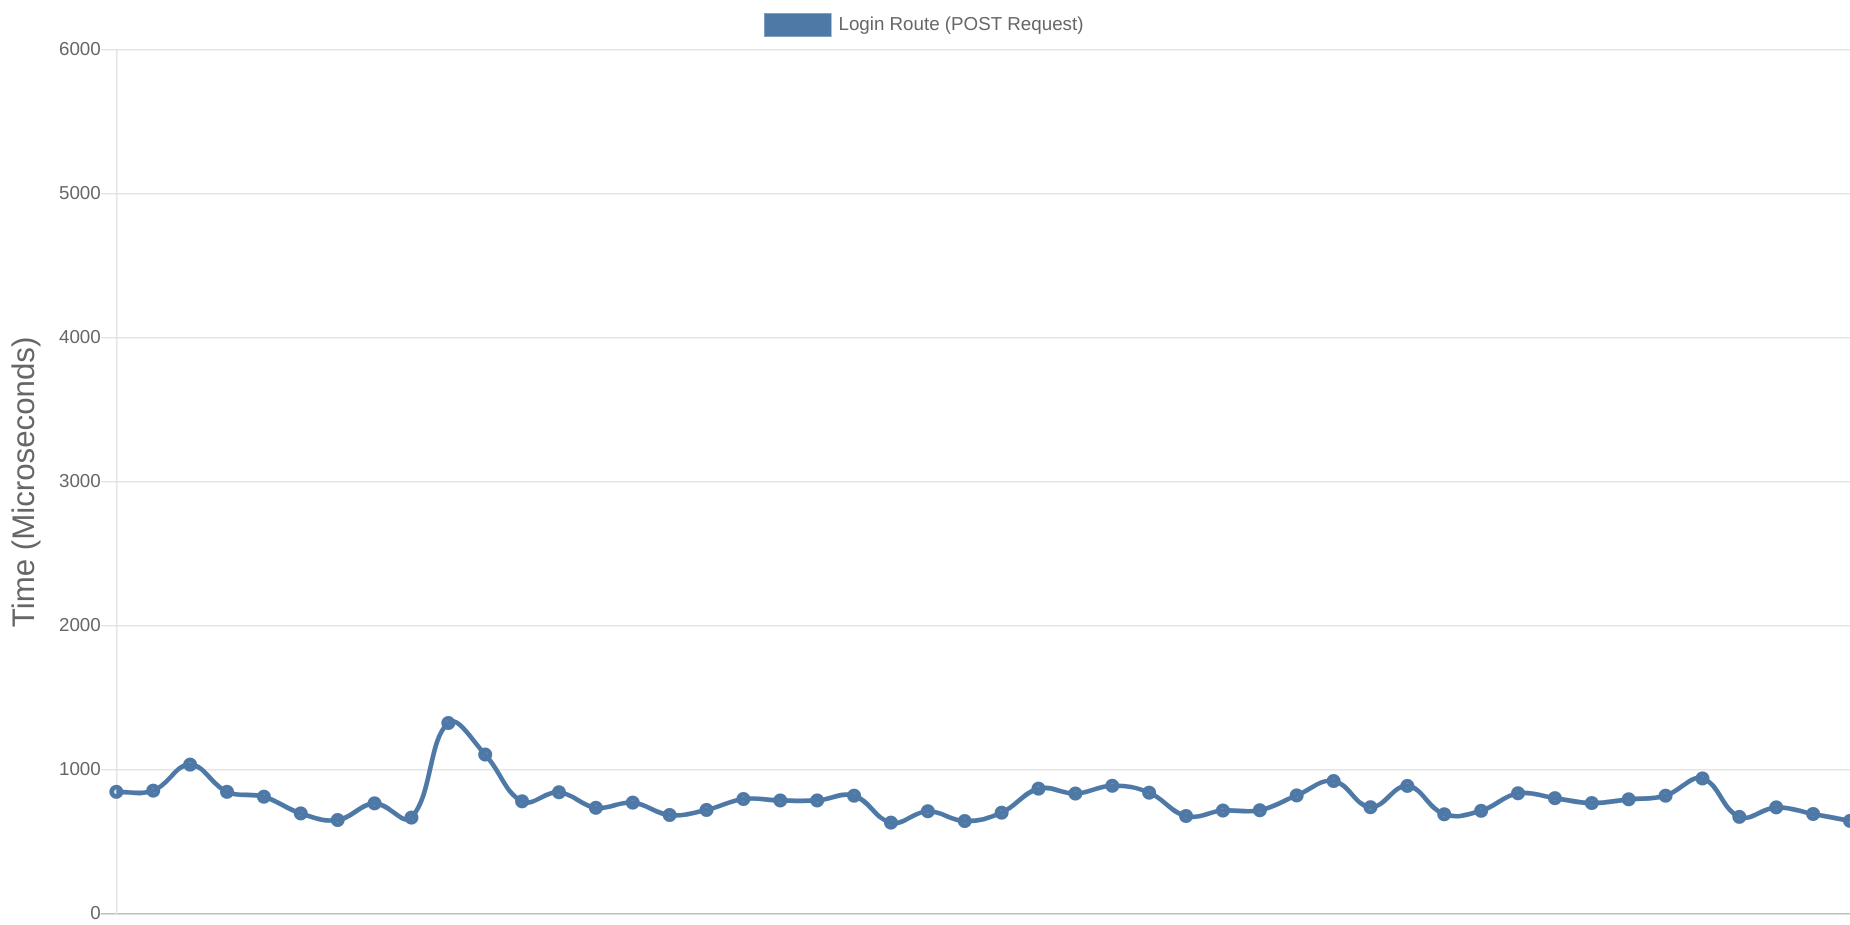
\includegraphics[width=\textwidth]{../results/login.png}
  \caption{/login route results}
  \label{login-test}
\end{figure}

This was very good to see, that my simplest service has a very consistent curve, sitting at around 700 microseconds, which is very fast. Most importantly it stayed fairly consistent throughout the testing with only 2 requests reaching over the 1000 microseconds barrier, I attribute these to system the system being under some load from other background processes.

\pagebreak
\subsubsection{/asset route}
The /asset route is a GET request that goes to the Hub service first. The hub requests the brain service for all its persistent storage needs, except for the ones that are cached. I have implemented caching using a Redis database and a strategy of storing the endpoint with some metadata as a key for the Redis database, if the key is present then we can serve cache. This is described in further detail above. The results for this request, are plotted in this figure \ref{asset-test}.

\begin{figure}[h!]
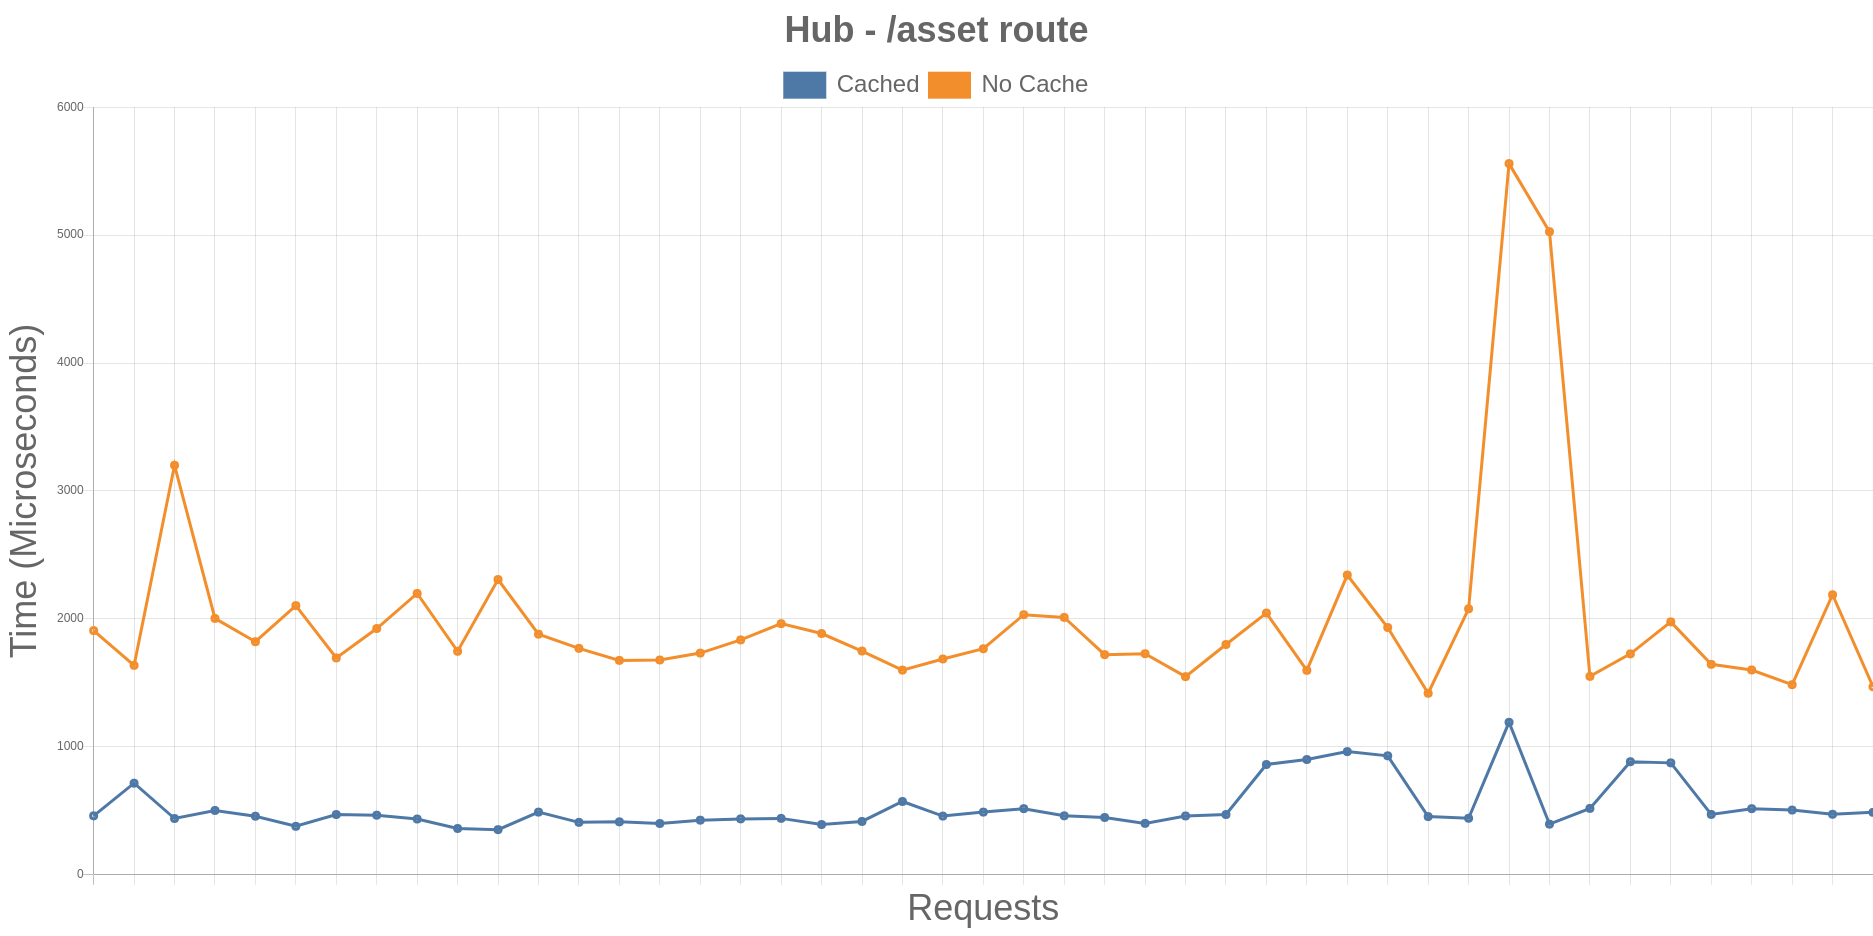
\includegraphics[width=\textwidth]{../results/asset.png}
  \caption{/asset route results}
  \label{asset-test}
\end{figure}

Starting with the non-cached results in orange, we can see that because the service has to make a request to the brain service and the brain then needs to perform a read from permanent storage from the PostgreSQL database, we end up with a much slower (but still very fast) turn around time. Averaging at around 2000 micro seconds, or just about 2 milliseconds. Noticeably there is a spike towards the end of the dataset, however this is an anomaly it seems and needs no further investigation, I attribute it to system noise. \\

The cached results are the most interesting ones, as you can see the request time averages at around 500 micro seconds (0.5 milliseconds), with a few spikes towards the end of the dataset, but averaging back down towards the end. This is significantly faster than requesting the brain for the information, 4 times faster in fact. This is extremely good to see that all the effort that went into creating an effective caching sub-system in the hub service has paid off.

\pagebreak
\subsubsection{/trade route}
This endpoint returns all the active trades in the system, a value that can be cached if the system is not under load and being used to actively trade, this would be especially useful when potential markets are closed or during periods of low activity. It is unlikely that I could achieve any sort of caching when the system is being used to constantly trade because the trades cache has to be constantly invalidated. The following test \ref{gettrade-test} does however test caching requests as well, but take into account this is only realistic to achieve during these periods of low activity.

\begin{figure}[h!]
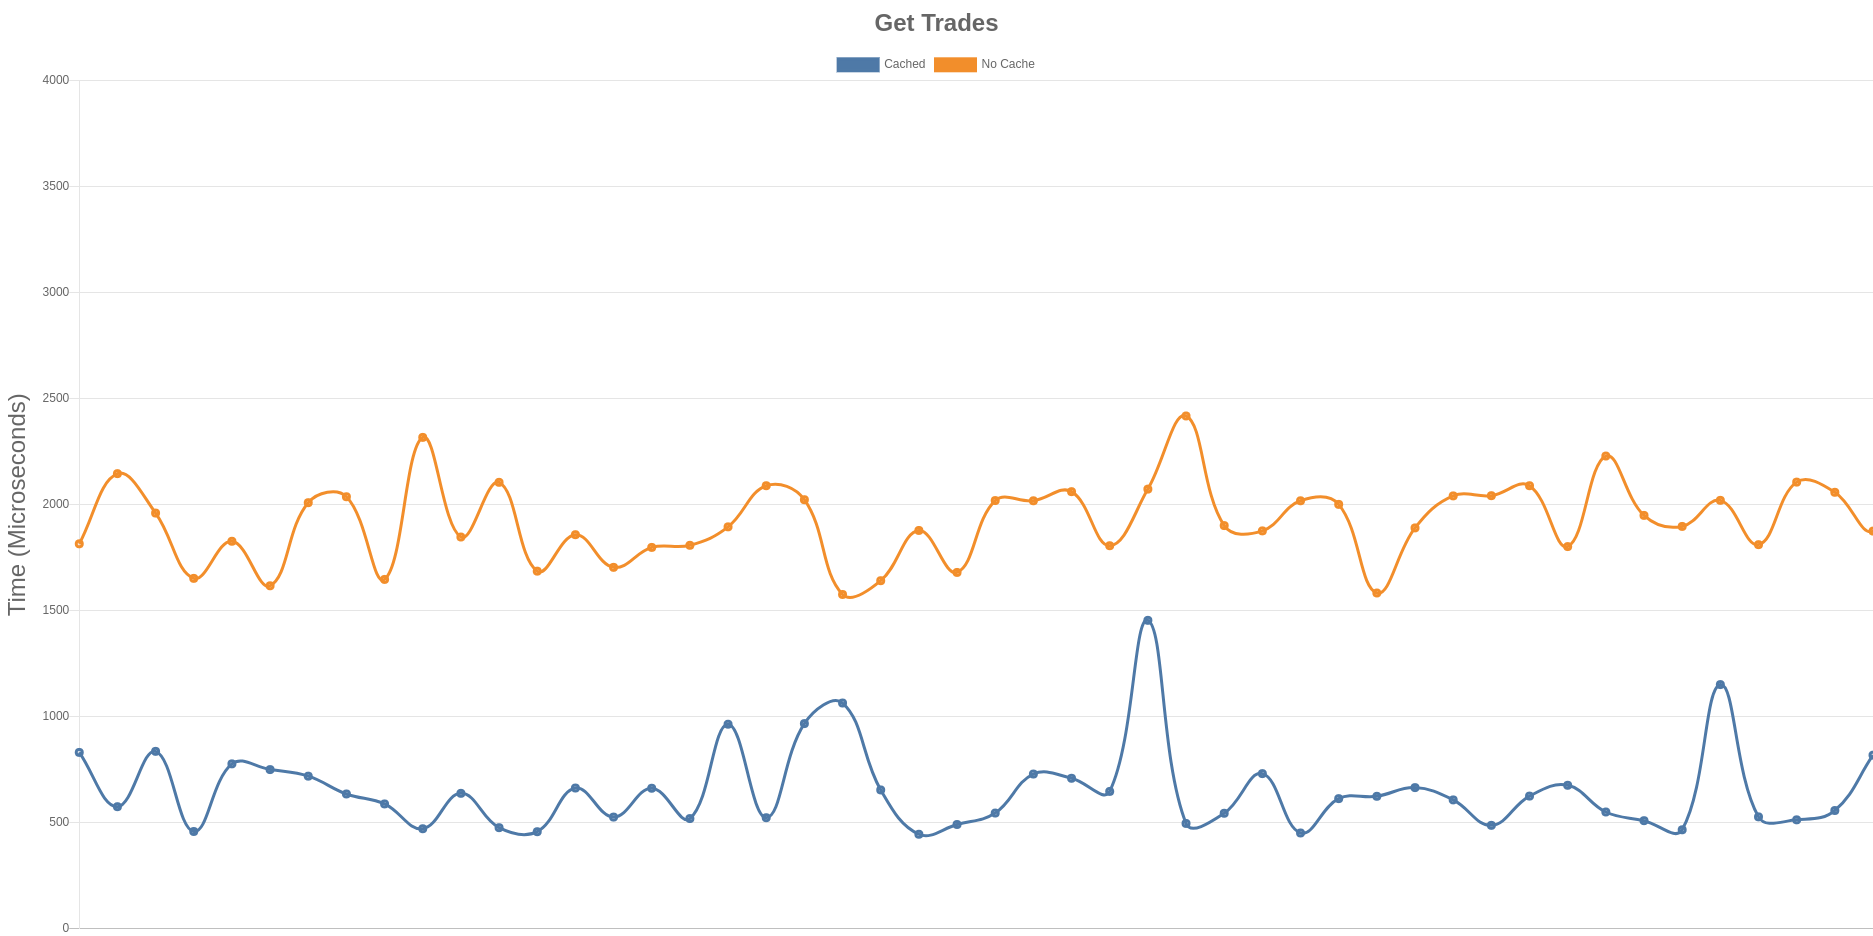
\includegraphics[width=\textwidth]{../results/get-trades.png}
  \caption{/trade/ route results}
  \label{gettrade-test}
\end{figure}

We see around the same improvement from cached results vs non-cached results when compared to the /asset endpoint results, an improvement of around 4 times. The average result for a cached request is around 600 microseconds, a number slightly higher than the assets because at any given point there are a lot more trades than there are assets, therefore the read from PostgreSQL naturally takes more time. \\

The non-cached results average at around 2000 microseconds (2 milliseconds), which is what I expected after testing the /asset endpoint.

\pagebreak
\subsubsection{/trade/create route}
This is a POST request to create a trade for a given asset, for a price. This can be a sell or buy transaction, but it is a fairly complicate endpoint because there is a lot of business logic that needs to happen. The system must check the user can trade this asset, or if they have enough money, as well as other general validation. It is also a request where basically no real caching is possible, and therefore the brain service takes almost all the load for this request. The results for the test are on the following figure \ref{create-trade}.

\begin{figure}[h!]
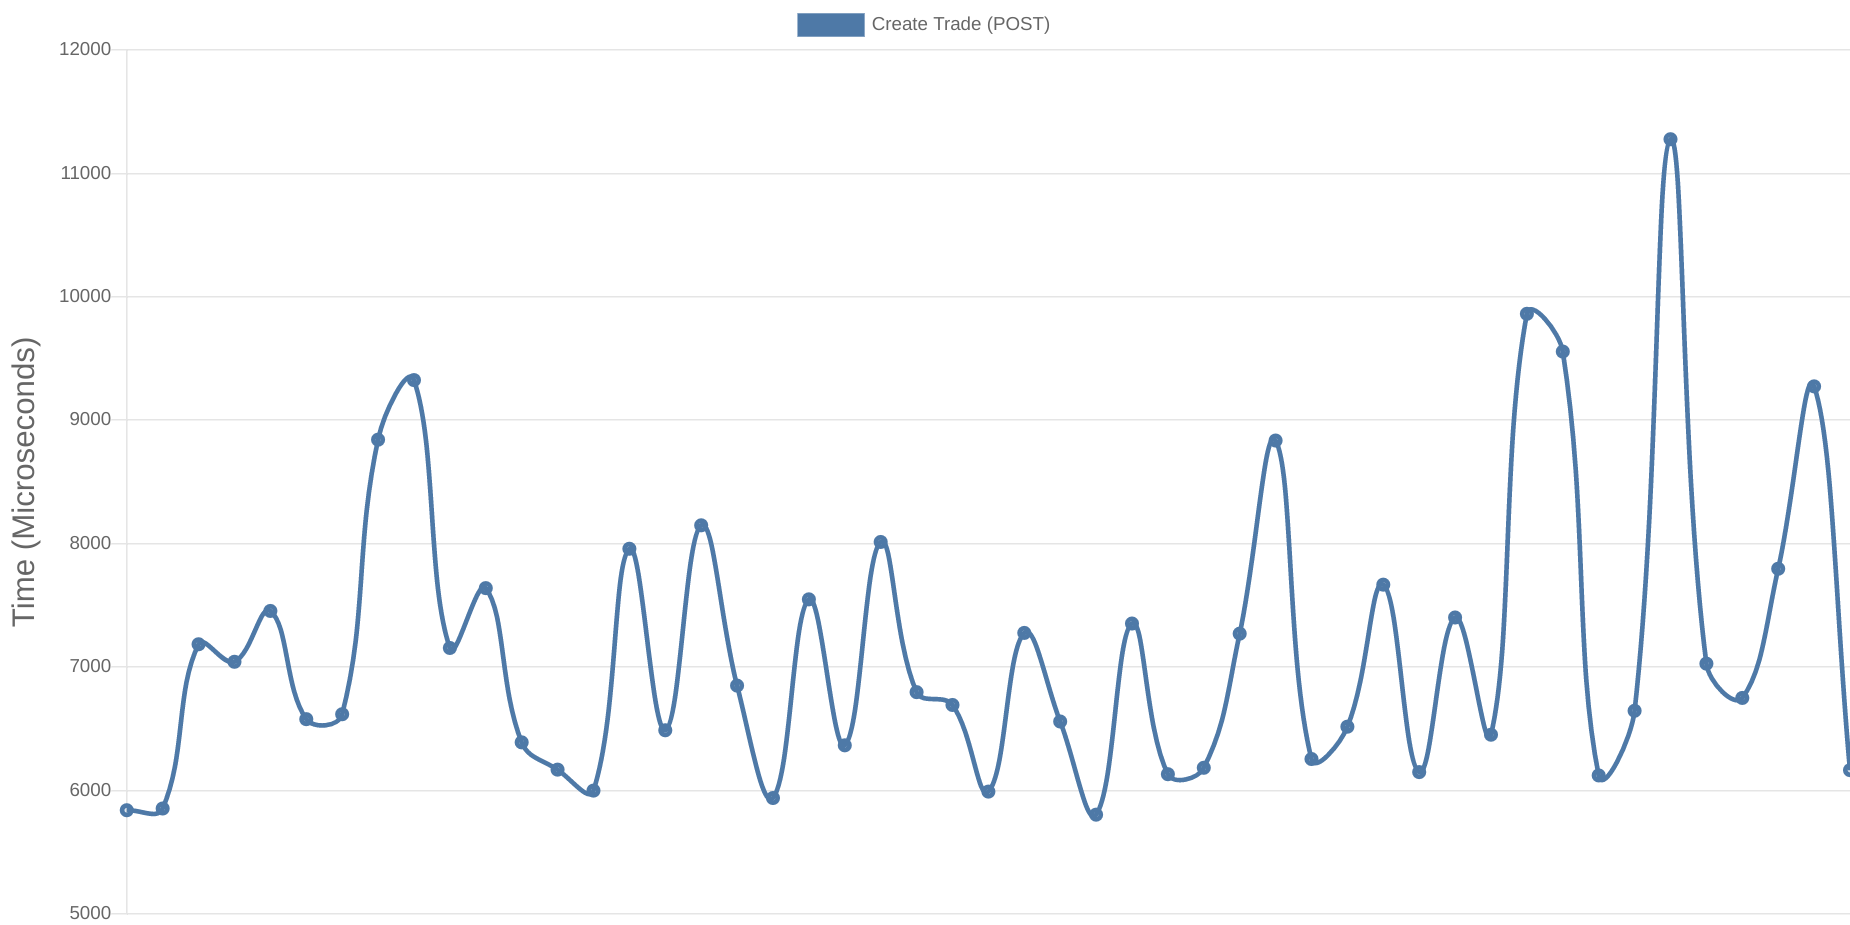
\includegraphics[width=\textwidth]{../results/create-trade.png}
  \caption{/trade/create route results}
  \label{create-trade}
\end{figure}

These results are much more chaotic, and naturally so because of how much more complex this endpoint is compared to other ones. We see the average at around 8000 microseconds (8 milliseconds), with quite a few data points that jump in terms of response time. I believe this is because of the lack of available threads on the virtual machine the test was conducted on, with around 4 threads some requests have to wait for others to finish before starting to handle the next one, hence explaining the jumps. This could be solved by having a better virtual machine (after all the one I am using isn't anything special). And then these results would look much more plausible. \\

\pagebreak
\subsubsection{/trade/complete route}
This endpoint is also a POST request, and it is very similar to the create trade endpoint, slightly less complex but still has to do a fair amount of validation in order to make sure that the transaction is a valid one (making sure the user has enough money, or enough of that asset, etc...). Again, no real caching is possible on this one and therefore I expect some more chaotic results. The results are plotted in the following figure \ref{create-trade-test}.

\begin{figure}[h!]
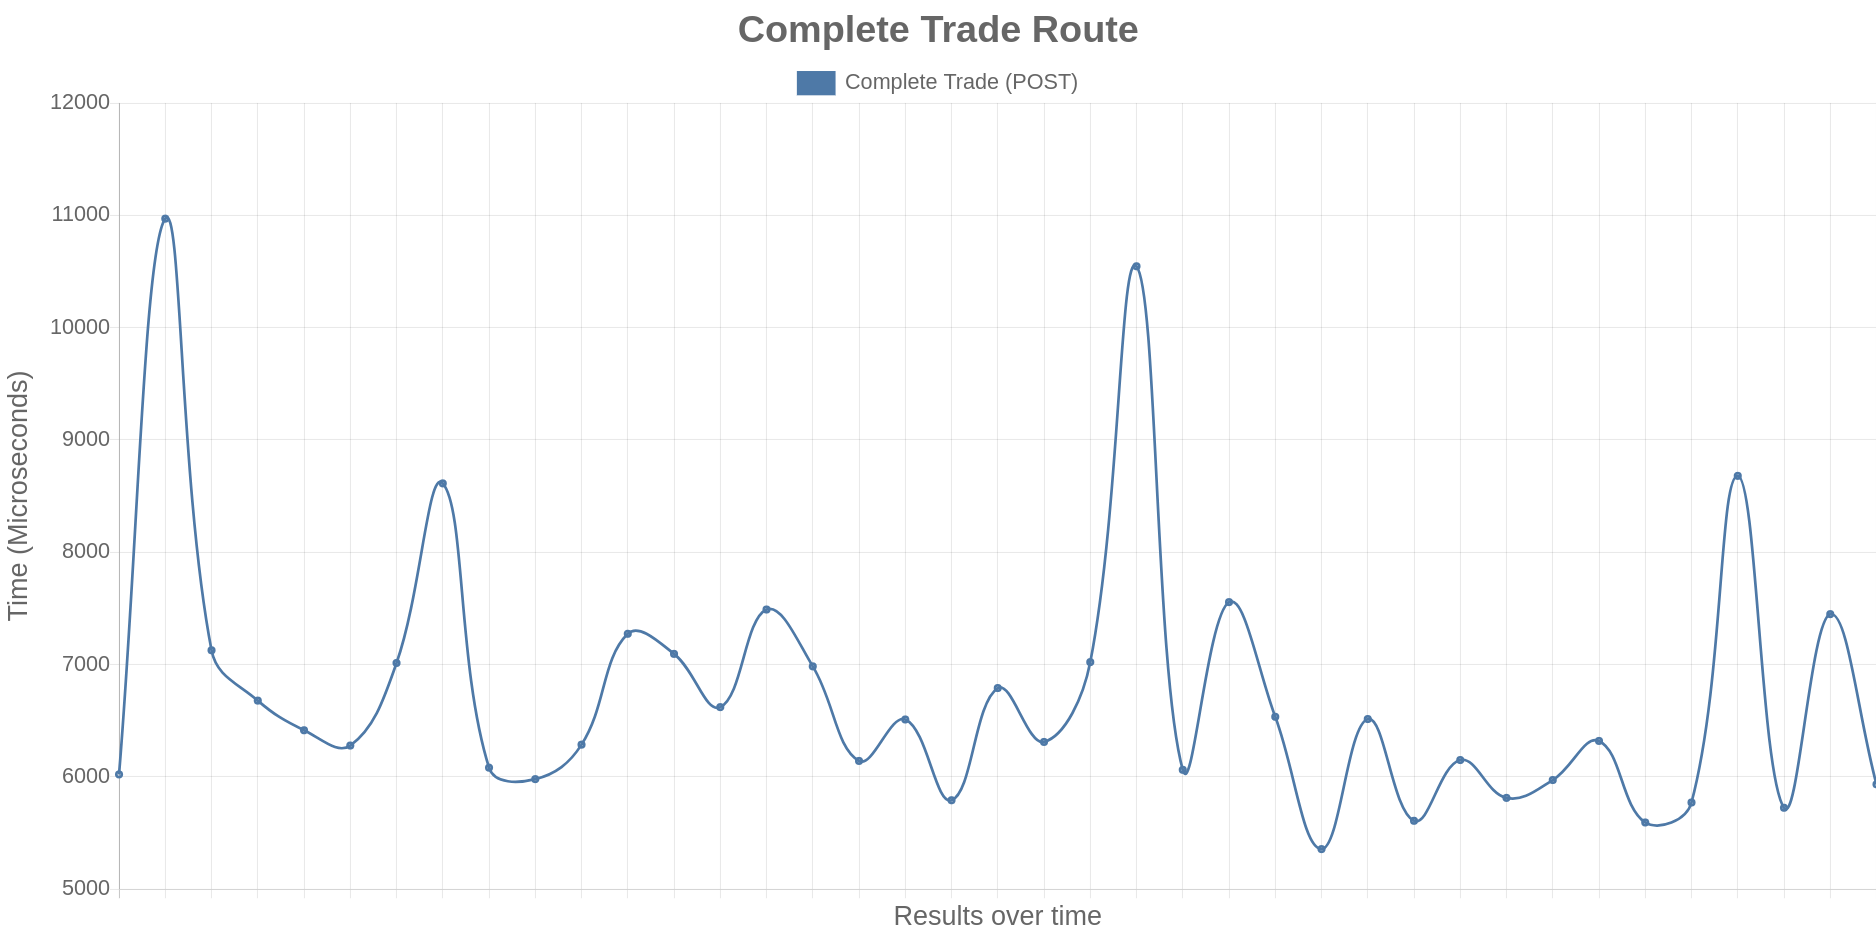
\includegraphics[width=\textwidth]{../results/complete-trade.png}
  \caption{/trade/create route results}
  \label{create-trade-test}
\end{figure}

These results are slightly less chaotic, due to the number of reads needed before being able to complete the transaction being less. Also the body is the request is significantly smaller than when you create a trade. We can see that the average is around 7000 microseconds (7 milliseconds), with only a few outliers where the system seems to have ran out of available threads. 

\subsection{End-to-End Performance}
I have mentioned before in the report that this type of testing is not very useful for my project because I do not have the resources to fully exhaust the system with my residential internet, and limited computational power. Nevertheless, I will still perform some tests to (hopefully) show that in my limited internet I cannot overpower the system. \\

To do this I will use a POST endpoints (/trade/create), which is the most CPU intensive end point in my system because it cannot be cached, and it needs to perform several validation checks before the user is allowed to actually create a trade. This figure \ref{e2e_route} shows the results and as we can see they are generally stable, with a few spikes in results, which I attribute to the machine temporarility  running out of threads to process the following request, but very quickly recovering. It is also worth noting that the virtual machine is running a whole operating system and therefore other processes could every once in a way require CPU time. \\

Just an extra note that this test is measured in milliseconds as opposed to the whitebox tests which are measured in microseconds, this means these tests take a significant amount of time, and seeing that in here \ref{create-trade} we have an average of 8 milliseconds, it seems that around 95\% of the end to end request comes from: Creating the request, sending the request, receiving it. This is why it is not feasible to use end-to-end testing to measure the performance is the system, because it does not fairly evaluate it.

\begin{figure}[h!]
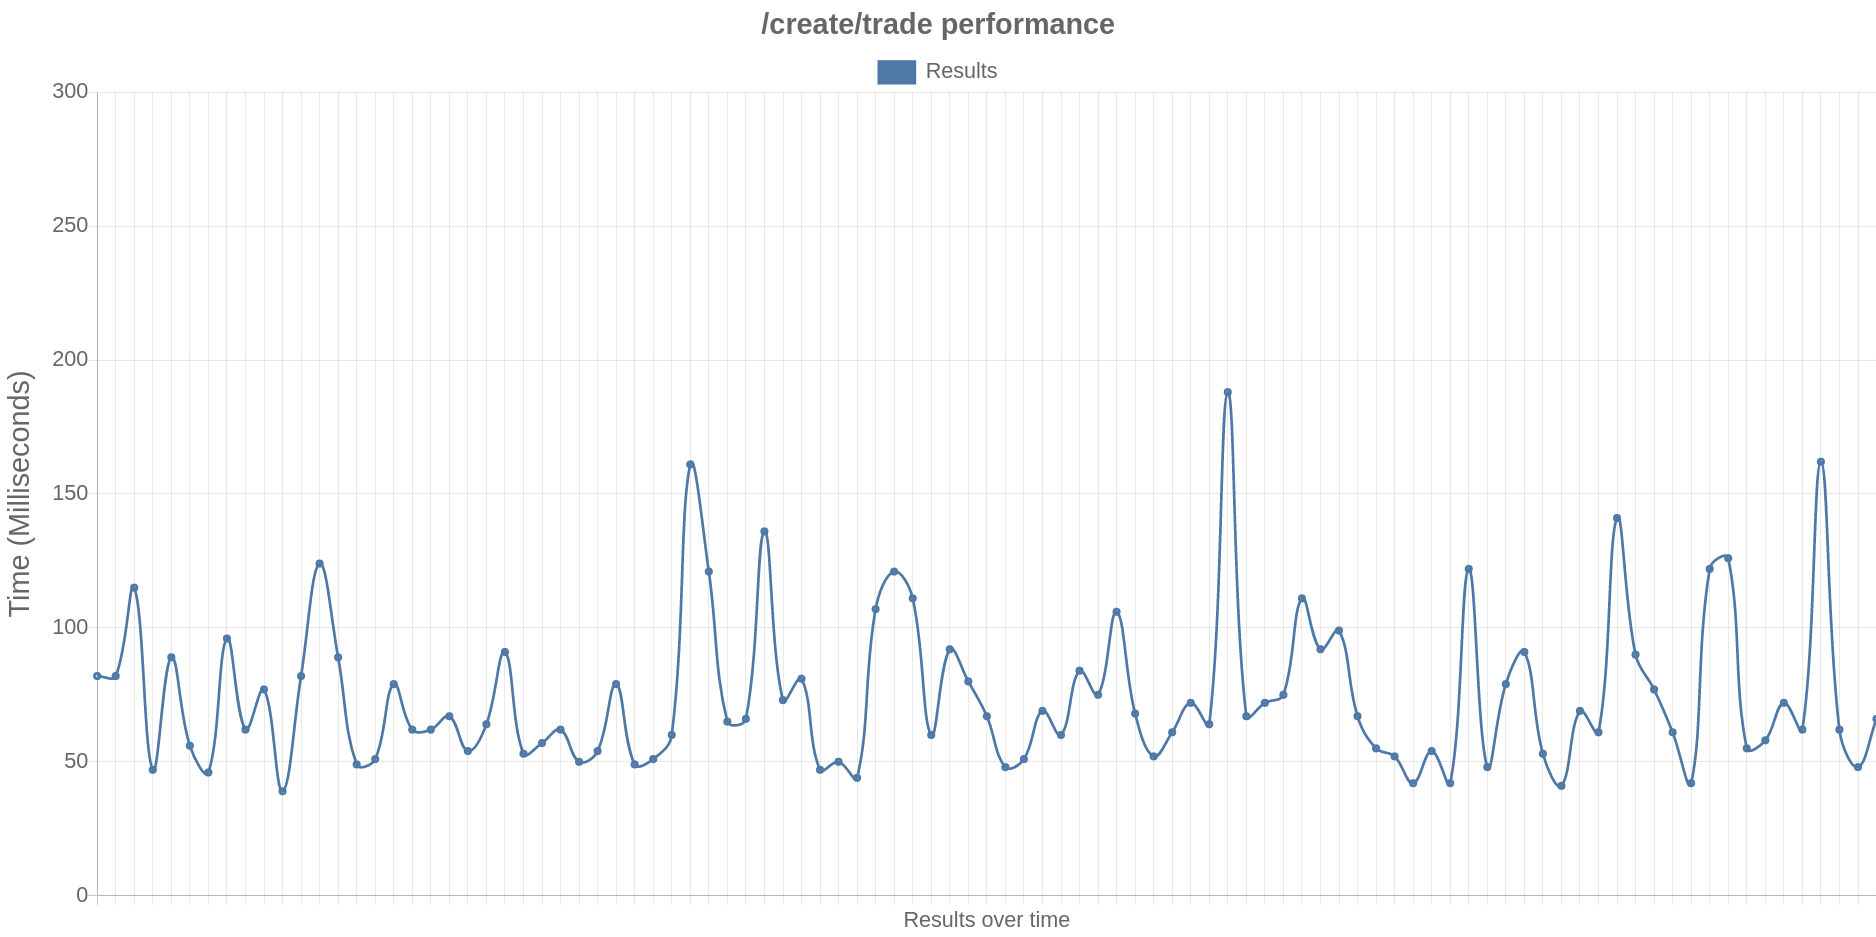
\includegraphics[width=\textwidth]{../results/e2e-createtrade.png}
  \caption{/trade/create route testing (End to end)}
  \label{e2e_route}
\end{figure}

\pagebreak
\section{Professional Issues}
There were a variety of professional issues that deal with topics that stretch beyond Computer Science. I discuss these below.

\subsection{Open Source}
I believe that any project must be extremely careful to use reputable tools to achieve their goals in the project, and I also believe that these tools should (in general), be open sourced. There are a few reasons for this, but the most important one is transparency. If you use a proprietary database system for example, you are at the mercy of the corporation, you are also restricted with how far you can extend the functionality of such software. Furthermore you tend to be a victim to Vendor Lock-in, discussed below. \\ 

There is a downside to using open source tools, and that is the fact that they don't have a warranty. If you make a mistake whilst using the open source tool there is no one obligated to help you solve the problem, nor is there anyone responsible except the engineer, if anything goes wrong.  \\

However, the open source community is very big and from what I found very helpful. The sheer quality of documentation of software I have used has helped me achieve my goals in this project tremendously. Furthermore, as soon as you use an open source tool, you also become a small part of this community, and can raise issues on the software, or even submit a pull request to fix these issues. 

\subsubsection{Licensing}
The license of open source software changes. Some open source projects cannot be used by individuals to create a product that is closed source, other projects do. The most flexible licenses, and therefore the only ones I have used are the following.

\begin{itemize}
  \item MIT~\cite{mit}
  \item Apache~\cite{apache}
  \item BSD~\cite{bsd}
\end{itemize}

All these licenses allow the use or software, free of charge, and to modify it freely and freely charge or use it in a proprietary product, the only restriction to some is that you cannot sell the exact software you are using from a license (You cant take an open source project and rebrand it and sell it), but obviously this isn't a problem in my project.

\subsection{Vendor Lock-in}
I mentioned above that you might become locked-in to a certain vendor when using proprietary software, the most common case for this comes with the hosting of your product. Typically engineers do not own big servers to host their products on and this was the case with me, so I had to resort to using some cloud service which is owned and managed by a big corporation. \\

I could have made this project a lot easier for me if I used technologies such as AWS Container Engine, or even AWS Lambdas, however these technologies lock you into only using the services of that certain cloud provider, and once you are in, it becomes very difficult to change your code so that it works somewhere else. Hence my decision to use only open source software in my project. \\

I happen to have had a friend with Azure credits and so I used a virtual machine in Azure. The reason for using a simple Linux virtual machine was because I wanted to avoid vendor lock in as much as possible, I could leave Azure whenever I want as long as I have another virtual machine on some other platform. The reason for this ease is because my entire system only needs a machine with docker engine running, which is also open source software that can run on any computer, this can be found on any major cloud provider.

\subsection{Data Safety}
My project uses only dummy data, however it is still important to consider the safety of the data that my system stores. This goal has to be thought of throughout the project, right from my decision to use PostgreSQL, the most popular relation database software in the world, which also happens to be open source (It also out performs all the competition by quite some margin). It was developed many decades ago and has some of the most reliable data storage mechanism of any database developed. This means that my data is safe, so long as I use transaction to store the data. \\

This also become an issue when developing my caching mechanism, because if you keep things in cache they are volatile and prone to being lost, therefore I made the decision to not cache any POST requests, and instead only cache the fetching of data, as this guarantees that the date will end up in the PostgreSQL database before any other place.

\pagebreak
\section{Final Evaluation}

And so my project concludes. I have learnt a lot from doing this project, specially how do develop distributed systems which is something I had never quite done before, I have also never really focused on performance in a backend project like I have in this one, and there was a lot of learning to do. \\

\subsection{Things that I planned correctly}
Generally, my planned risks were very correct. The platform performance and scalability being highlighted in my plan as the two main risks, and there were. However because of my well designed system with loosely coupled modules, I was able to make sure that each node was able to scale and work independently of the others, the separate database design also made this much easier. Furthermore the performance of the system is something I am very proud of, achieving sub 10 millisecond processing time for most requests, and some requests - through the use of caching going below the 1 millisecond mark is a much better result than I could have hoped for. I attribute this great performance to my ability to choose the correct tools for the job, it is clear to me now that Golang was the perfect language of choice, for dealing with distributed, networked systems such as the ones I developed, due to its very easy to use concurrency model, and effective garbage collection. \\

\subsection{Things that I didn't plan correct}

\subsubsection{BOTs}
In my plan I put a lot of emphasis on having BOTs trading across the network, when I realise now that this is was not going to help me massively improve the performance or stability of the system, it would have been interesting to see how the system would behave, and in some senses I have tested this, but the time it would have taken to create intelligent enough BOTs would have far outweighed the benefit to be gained, and would have bled over into an intelligent agent project, therefore during the development I choose to simply do basic API stress testing, using preset trades and assets without the need for intelligent agents. \\

\subsubsection{Development Time}
Furthermore, I severely underestimated the development time needed for the project. I mostly estimated the MVP development time correctly, and I did finish most of the development within Term 1, but I didn't account for the last 20\% of the project taking so long, this I should have been more aware of and could have made my timeline more realistic by giving myself more time for development. It is very common in the industry for the last 20\% to take longer than the first 80\% of the project.

\subsection{Conclusion}
My systems allows users to trade assets with other users. It seems innocent on the surface and could have been developed very quickly if I had no regard for performance and scalability. But with these concerns in mind I was able to make correct decisions in increasing the complexity of my project overall by splitting it into multiple parts (Micro services), and therefore allow for the individual scaling of each system. \\

The web interface for the project works seamlessly and is very responsive, and also has great UX (User experience) and UI (User interface) patterns that users are already familiar with.

\section{Bibliography}

\bibliography{ref}
\bibliographystyle{plain}

\pagebreak
\section{Logbook}

\textbf{29/09/2022} \\
First entry in the log book. This week I have taken the time to get organised, finalise my project idea and talk to my supervisor about it. I finalised the list of features that I wanted to have in the final product. Also got a draft of my plan.
\\

\noindent
\textbf{02/10/2022} \\
Finish the draft of the plan, but does not yet include the bibliography. Still need to walk through the marking grid and tick all the boxes.

\textbf{03/10/2022} \\
Completed the bibliography for now. However the work is not complete.

\textbf{05/10/2022} \\
Added testing, how currency will work and core and optional features to the plan.

\textbf{07/10/2022} \\
Finished the plan, submitting it today.

\textbf{11/10/2022} \\
Started implementing the "hub" service, which is the first point of contact from the user.

\textbf{12/10/2022} \\
Beginning template for the frontend application with all the dependencies installed.

\textbf{24/10/2022} \\
- Setup docker file for the hub micro service and a docker compose file to allow for easy deployment and development.
- Created a diagram for the overall system architecture.

\textbf{25/10/2022} \\
Connected frontend to the backend using websocket connection. I am still a week behind on my plan so I will have to work very hard this week to get back on schedule.

\textbf{31/10/2022} \\
Added RabbitMQ docker image, and created a test connection between hub and rabbitmq, it works.

\textbf{05/11/2022} \\
Setup the SQL schemas for the required databases.

\textbf{06/11/2022} \\
Started work on the authentication system.

\textbf{07/11/2022} \\
Finished register method in auth system, with some very nice code.
I also finished the login method.
Also finished the refresh method for JWTs. Basically did the entire Auth system.

\textbf{08/11/2022} \\
Connected frontend to backend login and register methods, learn about state management in SolidJs.

\textbf{23/11/2022} \\
I have a shared types library now and RPC communication working between hub and brain and sending back to the client. Need to implement the rest of the routes.

\textbf{26/11/2022} \\
There was a bug in the backend code, where some memory was declared in a different thread, and therefore was never updating, fixed it by redeclaring this memory.

\textbf{27/11/2022} \\
Fixed a lot of stuff on the backend and did some refactoring so some dependencies are shared. Also started the transactions endpoint but decided that I would like to connect the assets to the frontend first.

\textbf{29/11/2022} \\
 - Model methods to get user assets, create and complete transaction. Various bug fixes and connected the frontend to view assets. Some things are very prototypy, so will need refactoring
 - Endpoints for the trading of assets are complete, now I need further testing.

\textbf{29/11/2022} \\
 - All the backend is fully dockerised and running in containers!

\textbf{22/11/2022} \\
Started interim report, completed a first draft of the structure and included a lot of my research.

\textbf{23/11/2022} \\
Adding sections about version control monorepos and git worktrees.

\textbf{27/11/2022} \\
Section about project management

\textbf{30/11/2022} \\
Finished the first draft of the report!

\textbf{04/12/2022} \\
Finished integration testing app, it tests the authentication system and most of the routes on the hub.

\textbf{05/12/2022} \\
Final draft of the interim report completed

\textbf{02/12/2022} \\
Integration testing setup.

\end{document}
